\documentclass{article}
\newcommand{\R}{\textbf{R}}
\newcommand{\dee}{\;\text{d}}
\newcommand{\eps}{\varepsilon}
\newcommand{\pl}[2]{\frac{\partial #1}{\partial #2}}
\newcommand{\dl}[2]{\frac{\text{d} #1}{\text{d} #2}}
\newcommand{\sgn}{\text{sgn}}
\newcommand{\bigoh}{\mathcal{O}}
\usepackage{amsthm}
\newtheorem{thm}{Theorem}
\newtheorem{lem}{Lemma}
\newtheorem{dfn}{Definition}
\newtheorem{rmk}{Remark}
\newtheorem{cor}{Corollary}

\usepackage[left=3cm, right=3cm]{geometry}
\usepackage{parskip}
\usepackage{amssymb}
\usepackage{booktabs}
\usepackage{graphicx}
\usepackage[ruled,linesnumbered]{algorithm2e}
\usepackage{listings}
\usepackage{xcolor}
\usepackage{hyperref}

\newcommand{\maxvol}{{\texttt{maxvol}}}

\author{Jacob Hauck}
\title{Math 5601 Independent Study Project}
\date{}

\begin{document}
	\maketitle
	
	\section{Introduction}
	
	\minorheading{The problem with matrices}
	
	As we have seen throughout Math 5601, many numerical problems ultimately boil down to solving a system of linear equations $Ax = b$ for an unknown vector $x$. We also saw that most numerical methods for solving this problem involve performing many computations on the entries of the matrix $A$.
	
	Performing some process on a matrix $A$ is common outside of simply solving a linear system of equations, as matrices appear naturally in the analysis of many important and difficult problems. In many of these situations, the matrix $A$ might be enormous, and it may be necessary to process many such matrices. 
	
	In some cases, the vast majority of the entries of the matrix $A$ are zero, as we see in the final project, where the stiffness matrix has mostly zero entries. If this is the case, then the matrix is called \textbf{sparse}. Not all matrices one encounters are sparse, however. For example, to work with the samples on a uniform grid of a function defined on the unit cube $[0,1]^3$ with an apparently innocuous resolution of $\frac{1}{1000}$ effectively requires a stack of $1000$ separate $1000\times 1000$ matrices, which have altogether $10^9$ entries, which could consume the entirety of some systems' memory if each entry were stored as an individual, 64-bit, floating point number.
	
	If $A$ is a square $n \times n$ matrix\footnote{For simplicity, we focus on square matrices in complexity estimates, but matters are essentially the same with non-square matrices as well.}, then typical processes operating on $A$ require at least $\bigoh(n^2)$ operations. Indeed, simply storing a matrix in memory by creating a list of its entries already has $\bigoh(n^2)$ complexity, so it is no surprise that more complex operations incur at least as much time and memory as is required for storage alone.
	
	Considering that $n$ may be so large that the entries of the matrix might not even fit into available memory, it is clear that more efficient methods for performing computations on matrices are desirable, if not indispensable.
	
	\minorheading{Compressed representations}
	
	If a matrix is very sparse, in the sense that most of its entries are zero, we have no need to store all the entries. Instead, we can store only the nonzero entries, along with the locations of those entries. This can lead to an enormously compressed representation of a matrix, with the cost in time and memory of storing the matrix being $\bigoh(s)$, where $s$ is the number of nonzero entries. Moreover, if the format of the sparse data format is chosen intelligently, then many common matrix algorithms can be rewritten so that their memory costs are reduced from $\bigoh(n^2)$ to  $\bigoh(ns)$ (or lower); the reduction from quadratic cost in $n$ to something less than quadratic can lead to tremendous gains in performance, often making otherwise infeasible problems feasible (depending on how $s$ is related $n$, which varies by case).
	
	To give a simple example, computing the matrix-vector product $Ac$ of the $n\times n$ matrix and the $n\times 1$ column vector $c$ can be done in $\bigoh(n + s)$ operations if $A$ is known to havee only $s$ nonzero entries. Since this operation is used in many larger algorithms, like iterative solvers for the linear system $Ax = b$, we immediately see the significance of this performance gain. Other algorithms experience similar improvements.
	
	What, then, to do about matrices that are not sparse? Even if a matrix has no nonzero entries, it may still have a rank $r$ much lower than $n$. In this case, only $r$ of the columns (or rows) of the matrix are linearly independent; that is, the \textit{other} $n -r$ columns can be written as a linear combination of the $r$ linearly independent ones. By storing only the $r$ linearly independent columns and the $(n-r)r$ linear combination coefficients determining the other $n-r$ columns, the matrix can be stored with a time and memory cost of $\bigoh(nr)$.
	
	Again, depending on the relationship between $r$ and $n$, this reduction from quadratic to less than quadratic complexity in a basic operation like storage can lead to massive performance benefits in other algorithms. It can be beneficial, that is, \textit{if} the compressed data format can be used effectively with common matrix operations.
	
	This is all good and well if the matrix has a low rank, but what if the matrix has a high or full rank?
	
	\minorheading{Lossy compression}
	
	Even if a matrix is not sparse and not low-rank, we may still be able to approximate the matrix using a compressed representation (though representing it exactly may be off the table). In many cases, an approximation is sufficient, especially if we have a useful theoretical bound on the error of the approximation.
	
	Since the low-rank compressed representation didn't require sparsity but still achieved good compression, we might look to approximate a high-rank matrix by a low-rank one, then represent that low-rank approximation by an exact compressed form. This idea is intimately related to the following important and well-known theorem.
	
	\begin{thm} \textnormal{\bf(Singular value decomposition)}
		\label{thm:svd}
		Let $A \in \R^{n \times m}$. Then there exist orthogonal $U \in \R^{n\times n}$ and $V \in \R^{m\times m}$, and a matrix $\Sigma \in \R^{n\times m}$ defined by $\Sigma_{ii} = \sigma_i \ge 0$ for $1 \le i \le \min\{m,n\}$ and $\Sigma_{ij} = 0$ otherwise, such that
		\begin{equation}
			\label{eq:svd}
			A = U \Sigma V^T.
		\end{equation}
		Furthermore, the best rank-$r$ approximation of $A$ in both Frobenius and spectral norm is given by
		\begin{equation}
			\label{eq:truncated_svd}
			A' = U\Sigma' V^T,
		\end{equation}
		where $\Sigma'_{ij} = \Sigma_{ij}$ if $\max\{i,j\} \le r$, and $\Sigma'_{ij} = 0$ otherwise. Finally,
		\begin{equation}
			\lVert A - A'\rVert_2 = \sigma_{r+1}, \qquad \lVert A - A'\rVert_F = \left(\sum_{i > r} \sigma_i^2\right)^\frac{1}{2},
		\end{equation}
		where $\lVert \cdot \rVert_2$ and $\lVert \cdot \rVert_F$ are the spectral and Frobenius matrix norms, and we set $\sigma_{\min\{m,n\}+1} = 0$ by convention.
	\end{thm}
	
	This theorem gives us some idea as to how to construct a good, indeed, the \textit{best} (in some sense), approximation of $A$ by a low-rank matrix. The decomposition (\ref{eq:svd}) is called the \textbf{singular value decomposition (SVD)} of $A$, and (\ref{eq:truncated_svd}) is called the \textbf{(rank-$r$) truncated singular value decomposition} of $A$. The numbers $\{\sigma_i\}_{i=1}^{\min\{m,n\}}$ are called the \textbf{singular values} of $A$, and are unique up to permutation.
	
	Not only does Theorem \ref{thm:svd} provide an idea as to how to obtain a low-rank approximation, it also provides the \textit{exact value} of the error of such an approximation. This has made SVD a go-to tool in the approximation of matrices.
	
	One shortcoming of SVD, however, is that the matrices $U$ and $V$ can be difficult to interpret, and, in general, practical algorithms for computing the SVD of a square $n\times n$ matrix $A$ have a time complexity $\bigoh(n^2)$, which, as we have seen, may be problematic in some applications.
	
	\minorheading{A fast compression method}
	
	In the ideal scenario, we would like too have not only a compressed representation of a square $n\times n$ matrix $A$, we would also like to \textit{construct} that compressed representation efficiently. If the construction of the compressed representation is too slow, whatever process we want to do with our matrix may still be impossible. How, though, could we possibly do better than $\bigoh(n^2)$ time complexity in constructing an approximate representation of a square $n\times n$ matrix, considering that even storing such a matrix already requires $\bigoh(n^2)$ operations?
	
	Enter: submatrices. A submatrix is a smaller matrix formed from the elements of a larger matrix. A submatrix of a matrix $A$ can be used to form a low-rank approximation of the larger matrix through the so-called \textbf{pseudo-skeleton decomposition} \cite{goreinov_1997}. Although the pseudo-skeleton decomposition is, by Theorem \ref{thm:svd}, not the optimal low-rank approximation, we will see that it can still be pretty good.
	
	The main advantage that pseudo-skeleton decomposition enjoys over SVD is that it can be computed very quickly. Indeed, using the algorithm described in this paper, we will see that a rank-$r$ psuedo-skeleton decomposition can be computed in $\bigoh(nr^2)$ operations, which is significantly faster than SVD if $r$ is much smaller than $n$, and it is nearly as low as the $\bigoh(nr)$ cost of the resulting compressed representation.
	
	More importantly, because pseudo-skeleton decomposition only involves selecting elements from the original matrix to form a submatrix, it is not even necessary to know (or load into memory) every element of the original matrix. In other words, if the matrix being compressed has a good low-rank approximation, then a good pseudo-skeleton decomposition can be computed \textit{without event looking at the entire matrix}.
	
	In SVD, by contrast, every element of the $U$ and $V$ matrices depends on every element of the original matrix, so computing the SVD almost unavoidably involves looking at every entry of the original matrix. We also remark that the pseudo-skeleton decomposition is based on a submatrix, whose elements are just elements of the original matrix, which is easier to interpret than the more opaque $U$ and $V$ matrices in the SVD.
	
	In this project, we will investigate an algorithm known as \maxvol{} \cite{goreinov_2010}, whose purpose is to find a submatrix that is ``good enough'' for the corresponding pseudo-skeleton decomposition to approximate the original matrix well without incurring a computational cost of much greater complexity than is required to store the pseudo-skeleton decomposition (unlike truncated SVD). We will discuss the theory and motivation for the algorithm, provide a \texttt{NumPy} implementation\footnote{Full project code at \href{https://github.com/jacobhauck/MST-Coursework/blob/main/Math\%205601/Independent\%20Study\%20Project}{https://github.com/jacobhauck/MST-Coursework/blob/main/Math\%205601/Independent\%20Study\%20Project}}, and perform some numerical experiments to demonstrate the power of the algorithm.
	
	Before we move on, we remark that the theory and implementation in this project are woven together from various works, especially those of Goreinov, Oseledets, Tyrtyshnikov and others \cite{goreinov_1997, goreinov_2010, oseledets_2010a, olshevsky_2001, oseledets_2009, hamm_2022}. We provide one general citation here at the beginning, as many of the proofs and sections below draw on ideas from multiple sources and mix them with my own work to fill in their missing details and connect related results and concepts, making the citation of every specific idea overly complicated. Nevertheless, I have done my best to refer major results to the sources that seem most appropriate.
	
	\section{Theory}
	
	Before we can discuss what a pseudo-skeleton decomposition is and how to find one, we need introduce some notation for describing submatrices. We begin with a concise notation for referring to a set of indices in a matrix.
	
	\begin{dfn} \textnormal{\bf(Index slice)}
		\label{def:index_slice}
		Let $m \le n$, where $m$ and $n$ are integers. Define the \textbf{index slice from $m$ to $n$} by the sequence
		\begin{equation}
			m: n = \{i\}_{i=m}^n.
		\end{equation}
	\end{dfn}
	
	It will also be convenient to have a concise notation for the standard basis vectors.
	
	\begin{dfn} \textnormal{\bf(Standard basis)}
		\label{def:standard_basis}
		Let $e_j \in \R^n$ denote the $j$th standard basis vector in $\R^n$, defined by
		\begin{equation}
			(e_j)_i = \begin{cases}
				1 & i = j, \\
				0 & i \ne j.
			\end{cases}
		\end{equation}
		Be aware that we will reuse the symbol $e_j$ for different values of $n$, sometimes in the same context.
	\end{dfn}
	
	Next, we give a formal definition of a submatrix. We will frequently need to use both the submatrix itself in matrix formulas and its corresponding row and column indices, so we define a compact indexing notation relating a matrix and the submatrix along given rows and columns.
	
	\begin{dfn} \textnormal{\bf(Submatrix)}
		\label{def:submatrix}
		Let $A \in \R^{m\times n}$ be a matrix. Let $I = \{I_i\}_{i=1}^r$ be a sequence of distinct row indices of $A$, and let $J = \{J_j\}_{j=1}^c$ be a sequence of distinct column indices of $A$. The \textbf{submatrix of $A$ with rows $I$ and columns $J$} is the matrix $A(I,J) \in \R^{r\times c}$ with entries
		\begin{equation}
			[A(I,J)]_{ij} = A_{I_iJ_j}.
		\end{equation}
		If the special symbol $:$ is used as row indices or column indices, it means the entire sequence $1:m$ or $1:n$.
		
		If $I$ or $J$ is a single integer $i$ or $j$ instead of a sequence, we take this to mean $I = i:i$ or $J = j:j$, the sequence consisting of that one integer.
	\end{dfn}
	
	\subsection{Skeleton Decomposition}
	
	The following is a simple theorem about matrix multiplication with submatrices; it is trivial, but we will use it many times in the subsequent proofs, and it also serves as the motivation for the form of the pseudo-skeleton decomposition.
	
	\begin{lem} \textnormal{\bf(Submatrix of a product)}
		\label{lem:submatrix_prod}
		Let $A\in \R^{m\times r}$, and let $B\in \R^{r\times n}$. Then for any row indices $I$ of $A$,
		\begin{equation}
			(AB)(I,:) = A(I,:)B,
		\end{equation}
		and for any column indices $J$ of $B$,
		\begin{equation}
			(AB)(:,J) = AB(:,J).
		\end{equation}
	\end{lem}
	
	\begin{proof}
		Observe that
		\begin{equation}
			[(AB)(I,:)]_{ij} = (AB)_{I_ij} = \sum_{k=1}^rA_{I_ik}B_{kj} = \sum_{k=1}^rA(I,:)_{ik}B_{kj} = [A(I,:)B]_{ij}, \quad i\in 1:m,\; j\in 1:n,
		\end{equation}
		so $(AB)(I,:) = A(I,:)B$.
		
		Similarly,
		\begin{equation}
			[(AB)(:,J)]_{ij} = (AB)_{iJ_j} = \sum_{k=1}^rA_{ik}B_{kJ_j} = \sum_{k=1}^rA_{ik}B(:,J)_{kj} = [AB(:,J)]_{ij}, \quad i\in 1:m,\; j\in 1:n,
		\end{equation}
		so $(AB)(:,J) = AB(:,J)$.
	\end{proof}

	\colorlet{col:submat}{green!70!black}	
	This simple result makes it easy to construct a low-rank matrix that agrees with a given submatrix on the \textbf{cross} of the submatrix, which are the entries in the original matrix in the same row or column as any entry in the submatrix. To give a concrete example, suppose that
	\begin{equation}
		A = \left[\begin{matrix}
			A_{11} & {\color{col:submat}A_{12}} & A_{13} & A_{14} & {\color{col:submat}A_{15}} \\
			A_{21} & A_{22} & A_{23} & A_{24} & A_{25} \\
			A_{31} & A_{32} & A_{33} & A_{34} & A_{35} \\
			A_{41} & {\color{col:submat}A_{42}} & A_{43} & A_{44} & {\color{col:submat}A_{45}} \\
			A_{51} & A_{52} & A_{53} & A_{54} & A_{55}
		\end{matrix}\right],
	\end{equation}
	and consider the submatrix on the  entries
	\begin{equation}
		A((1,4), (2, 5)) = \left[\begin{matrix}
			\color{col:submat}A_{12} & \color{col:submat}A_{15} \\
			\color{col:submat}A_{42} & \color{col:submat}A_{45}
		\end{matrix}\right].
	\end{equation}
	Using this submatrix, we can easily apply Lemma \ref{lem:submatrix_prod} to construct a low-rank approximation $S$ (we will see how shortly in Theorem \ref{thm:skeleton_submatrix_exact}) that agrees with $A$ on the cross of the submatrix. In other words, coloring every entry of $S$ green that agrees with $A$, we have
	\begin{equation}
		\label{eq:cross_approximation_demo}
		S = \left[\begin{matrix}
			\color{col:submat} A_{11} & \color{col:submat} A_{12} & \color{col:submat} A_{13} & \color{col:submat} A_{14} & \color{col:submat} A_{15} \\
			S_{21} & \color{col:submat} A_{22} & S_{23} & S_{24} & \color{col:submat} A_{25} \\
			S_{31} & \color{col:submat} A_{32} & S_{33} & S_{34} & \color{col:submat} A_{35} \\
			\color{col:submat} A_{41} & \color{col:submat} A_{42} & \color{col:submat} A_{43} & \color{col:submat} A_{44} & \color{col:submat} A_{45} \\
			S_{51} & \color{col:submat} A_{52} & S_{53} & S_{54} & \color{col:submat} A_{55}
		\end{matrix}\right].
	\end{equation}
	
	From this, it is evident that $S$ agrees with $A$ on the row and column emanating from every element in the submatrix $A((1,4),(2,5))$; this is where the name ``cross'' comes from.
	
	To construct $S$, we simply take the columns of the submatrix and the rows of the submatrix and put the inverse in between. When we apply Lemma \ref{lem:submatrix_prod}, we see that $S$ and $A$ agree on the cross of the submatrix.
	
	\begin{thm}
		\label{thm:skeleton_submatrix_exact}
		Let $A \in \R^{m\times n}$. If $A(I,J) \in \R^{r\times r}$ is a square submatrix of $A$ with rank $r$, and $S = A(:,J)A(I,J)^{-1}A(I,:)$, then
		\begin{equation}
			\label{eq:skeleton_submatrix_exact}
			A(I,:) = S(I,:), \qquad A(:,J) = S(:,J).
		\end{equation}
	\end{thm}
	
	\begin{proof}
		By Lemma \ref{lem:submatrix_prod},
		\begin{equation}
			S(I,:) = (A(:, J)GA(I,:))(I,:) = A(I,J)A(I,J)^{-1}A(I,:) = A(I,:),
		\end{equation}
		and
		\begin{equation}
			S(:,J) = (A(:, J)GA(I,:))(:,J) = A(I,:)A(I,J)^{-1}A(I,J) = A(:, J).
		\end{equation}
	\end{proof}
	
	To give a more fanciful interpretation of the green rows and columns in (\ref{eq:cross_approximation_demo}), we can think about them as the ``bones'' of the matrix $A$, in the sense that they contain most of the essential ``structure'' of the matrix. 
	
	Indeed, if $A$ has the same rank as the submatrix $S$, then $S$ and $A$ are in fact identical, meaning that essentially all the information in $A$ is contained in the submatrix, which provides a highly compressed representation of the original matrix. In this case, the representation $S$ is known as the \textbf{skeleton decomposition} of the matrix, after the bone analogy above.
	
	\begin{thm}
		\label{thm:skeleton_decomposition} \textnormal{\bf(Skeleton decomposition)}
		Let $A \in \R^{m\times n}$ be a matrix with rank $r$. If $A(I,J) \in \R^{r\times r}$ is a square submatrix of $A$ with rank $r$, then
		\begin{equation}
			\label{eq:skeleton}
			A = A(:,J)A(I,J)^{-1}A(I,:).
		\end{equation}
		This factorization is called a \textbf{skeleton decomposition}\footnote{Since $C = A(:,J)$ is a matrix of columns of $A$, and $R = A(I,:)$ is a matrix of rows of $A$, if we define $U = A(I,J)^{-1}$, then the corresponding skeleton decomposition is given by $A = CUR$, which is where the common alternative name ``CUR decomposition'' comes from. We remark that CUR decomposition is obviously a much more boring name. On the other hand, the term ``skeleton decomposition'' is not nearly as safe for Googling...} of $A$.
	\end{thm}
	
	\begin{proof}
		The columns of $A$ at indices $J$ (that is, $\{A(:, J_j)\}_{j=1}^r$) are linearly independent because
		\begin{equation}
			\sum_{j=1}^r\alpha_j A(:, J_j) = 0 \implies \sum_{j=1}^r \alpha_j A(I, J_j) = 0 \implies\alpha_j = 0, \quad j \in 1:r
		\end{equation}
		because the columns $\{A(I,J_j)\}_{j=1}^r$ of $A(I,J)$ must be linearly independent by the fact that $A(I,J)$ has rank $r$.
		
		Thus, since $A$ has rank $r$, every other column of $A$ must be a linear combination of the columns at indices $J$. That is, there exists $\{\alpha_{\ell j}\}$ for $j \in 1:r$ and $\ell\in 1:n$ such that
		\begin{equation}
			A(:, \ell) = \sum_{j=1}^r \alpha_{\ell j} A(:, J_j).
		\end{equation}
		Define $\varphi : \R^r \to \spn\{A(:, J_j) \mid j \in 1:r\}$ by $\varphi(e_j) = A(:,J_j)$. Clearly, $\varphi$ is linear and onto. By the linear independence of $\{A(:,J_j)\}$, $\varphi$ maps an $r$-dimensional space onto an $r$-dimensional space, so $\varphi$ must also be one-to-one. Thus, $\varphi$ is invertible, with $\varphi^{-1}(A(:, J_j)) = e_j$ for $j \in 1:r$.
		
		Let $x \in \R^n$. Viewing $A$ and $A(I,J)$ as linear mappings defined by matrix-vector multiplication, we have
		\begin{align}
			(A(I,J)\circ \varphi^{-1} \circ A)(x) &= (A(I,J)\circ\varphi^{-1})\left(\sum_{\ell=1}^nA(:, \ell)x_\ell\right) = \sum_{\ell=1}^nx_\ell A(I,J)\varphi^{-1}(A(:,\ell)) \\
			&=\sum_{\ell=1}^nx_\ell A(I,J)\varphi^{-1}\left(\sum_{j=1}^r\alpha_{\ell j}A(:,J_j)\right)\\
			&=\sum_{\ell=1}^nx_\ell A(I,J)\sum_{j=1}^r\alpha_{\ell j} e_j =\sum_{\ell=1}^nx_\ell \sum_{j=1}^r\alpha_{\ell j}A(I, J_j)\\
			&= \sum_{\ell=1}^nx_\ell\left(\sum_{j=1}^r\alpha_{\ell j}A(:,J_j)\right)(I,:) = \sum_{\ell=1}^n A(I, \ell) x_\ell \\
			&= A(I, :)x.
		\end{align}
		Since $x$ was arbitrary, and $A(I,J)$ and $\varphi^{-1}$ are invertible, it follows that
		\begin{equation}
			A = \varphi \circ A(I,J)^{-1}\circ A(I,:)
		\end{equation}
		as a linear map. 
		
		For any $x \in \R^n$, we can write $A(I,J)^{-1}A(I,:)x$ as a linear combination of $\{e_j\}_{j=1}^r$; that is, there exists $\{\beta_j\}$ such that
		\begin{equation}
			A(I,J)^{-1}A(I,:)x = \sum_{j=1}^r\beta_j e_j.
		\end{equation}
		Then
		\begin{equation}
			Ax = \varphi\left(\sum_{j=1}^r\beta_je_j\right) = \sum_{j=1}^r\beta_j A(:,J_j) = A(:,J)\sum_{j=1}^r\beta_je_j = A(:,J)A(I,J)^{-1}A(I,:)x.
		\end{equation}
		Since $x$ was arbitrary, (\ref{eq:skeleton}) follows.
	\end{proof}
	
	
	\minorheading{Pseudo-skeleton decomposition}
	
	The skeleton decomposition gives us a way to represent a rank-$r$ matrix that only requires us to know that entries of the matrix in the rows $I$ and columns $J$, which means $2nr$ entries, if the matrix is $n\times n$. This is that all-important property that we were looking for: avoiding the necessity to use all the entries of the matrix.
	
	Unfortunately, we still need a way to find those $2nr$ entries efficiently. More importantly, though, skeleton decomposition requires us to know the rank of the matrix, and it doesn't allow us to approximate a high-rank matrix by a low-rank one.
	
	Even so, by Theorem \ref{thm:skeleton_submatrix_exact}, a rank-$r$ submatrix may still be used to represent the original matrix on the cross of the submatrix, even if the original matrix has higher than $r$. This leads to the natural question (and the title of our main reference \cite{goreinov_2010}): can we choose a ``good enough'' submatrix so that the matrix $S$ in Theorem \ref{thm:skeleton_submatrix_exact} not only agrees with $A$ on the cross, but also approximates $A$ \textit{off} of the cross?
	
	To facilitate the discussion of this question, we need to introduce the formal concept of pseudo-skeleton decomposition, which is a generalization of the skeleton decomposition\footnote{We remark that the pseudo-skeleton decomposition is not really a decomposition in the sense that it provides an exact factorization of the matrix; rather, it is a factorized \textit{approximation} of the matrix. For this reason, some authors instead call it a ``pseudo-skeleton approximation'' or ``pseudo-skeleton component'' of the matrix \cite{goreinov_1997, oseledets_2010a}.}.
	
	\begin{dfn} \textnormal{\bf(Pseudo-skeleton decomposition)}
		Let $A \in \R^{m\times n}$ be a matrix, and let $I$ and $J$ be sequences of row indices of $A$ of length $r$. If $G \in \R^{r\times r}$, then
		\begin{equation}
			B = A(:, J) G A(I,:)
		\end{equation}
		is called a \textbf{pseudo-skeleton decomposition} of $A$ with \textbf{core} $G$, \textbf{row indices $I$}, and \textbf{column indices $J$}.
	\end{dfn}
	
	Now the question we need to answer, and the main focus of this analysis, is this: can we choose the core $G$ and submatrix $A(I,J)$ so that the pseudo-skeleton approximation is nearly as good as the best rank-$r$ approximation? At this point, we will fix $G = A(I,J)^{-1}$ (and assume that $A(I,J)$ is invertible) after the skeleton approximation. This will allow us to focus on simply finding a good enough submatrix $A(I,J)$. Moreover, retaining the form of the skeleton decomposition means that we will also avoid having to use all the entries $A$ to find the pseudo-skeleton decomposition, just as we observed in the case of skeleton decomposition.
	
	\subsection{A Good Submatrix: Existence and Criteria}
	
	The first step in our analysis is to show that a pseudo-skeleton decomposition can be a good low-rank approximation. This analysis will lead naturally to the next step, which in turn will lead to the construction of the pseudo-skeleton decomposition algorithm.
	
	The proof of the existence of a good pseudo-skeleton decomposition with our choice of $G = A(I,J)^{-1}$ is fairly technical, but I will try to give some motivation for the key ideas nonetheless. 
	
	\minorheading{Motivation}
	
	To quantify what we mean by a good pseudo-skeleton decomposition, we introduce a norm in which to measure the error.
	
	\begin{dfn} \textnormal{\bf(Chebyshev Norm)}
		\label{def:chebyshev_norm}
		If $A \in \R^{m\times n}$, define the \textbf{Chebyshev norm} of $A$ by
		\begin{equation}
			\label{eq:chebyshev_norm}
			\chebnorm{A} = \max_{i,j} |A_{ij}|.
		\end{equation}
	\end{dfn}
	
	We want to show that there is a pseudo-skeleton decomposition such that the error in Chebyshev norm is not too much bigger than the error of the best low-rank approximation. In other words, we want to show that if $A(I,J)$ is a ``good'' rank-$r$ submatrix, then
	\begin{equation}
		\label{eq:theory_goal}
		\chebnorm{A - A(:J)A(I,J)^{-1}A(J,:)} \lesssim \sigma_{r+1},
	\end{equation}
	where $\sigma_{r+1}$ is the $(r+1)$-th largest singular value of $A$, which is the same as the error of the best rank-$r$ approximation of $A$ in the spectral norm by Theorem \ref{thm:svd}.
	
	The Chebyshev error is the maximum absolute difference of the elements of the matrices, which is a natural way to measure error. The spectral norm is natural as well, in its own way, but we will see that it is easier to control the error of a particular element of a pseudo-skeleton decomposition than it is to control the spectral norm error of the entire decomposition.
	
	In any case, all matrix norms are equivalent, and the spectral norm can be optimally controlled by the Chebyshev norm as follows.
	
	\begin{lem}
		\label{lem:chebyshev_estimate}
		For any matrix $A \in \R^{m\times n}$,
		\begin{equation}
			\euc{A} \le \sqrt{mn}\chebnorm{A}
		\end{equation}
		where $\euc{\cdot}$ is the spectral norm. This inequality is sharp.
	\end{lem}
	
	\begin{proof}
		Let $x \in \R^n$. Overloading $\euc{\cdot}$ to also mean the Euclidean vector norm in $\R^n$, the Cauchy-Schwarz inequality implies that
		\begin{equation}
			\euc{Ax} = \sqrt{\sum_{i=1}^m|Ax_i|^2} = \sqrt{\sum_{i=1}^m\left|\sum_{j=1}^nA_{ij}x_j\right|^2} \le \sqrt{\sum_{i=1}^m\left(\sum_{j=1}^n|A_{ij}|^2\right)\left(\sum_{j=1}^n|x_j|^2\right)}.
		\end{equation}
		By definition, $|A_{ij}|^2 \le \chebnorm{A}^2$, so
		\begin{equation}
			\euc{Ax} \le \sqrt{\sum_{i=1}^m n\chebnorm{A}^2\euc{x}^2} = \sqrt{mn}\chebnorm{A}\euc{x}.
		\end{equation}
		If $\euc{x} \ne 0$, then
		\begin{equation}
			\frac{\euc{Ax}}{\euc{x}} \le \sqrt{mn}\chebnorm{A}.
		\end{equation}
		Taking the supremum over $x \ne 0$ on both sides completes the proof of the inequality.
		
		For the sharpness, take $x\in \R^n$ such that $x_j = n^{-\frac{1}{2}}$ for $j \in 1:n$, so that $\euc{x} = 1$, and take $A \in \R^{m\times n}$ such that $A_{ij} = 1$ for all $i,j$. Then $\chebnorm{A} = 1$, and
		\begin{equation}
			\euc{Ax} = \sqrt{\sum_{i=1}^m\left|\sum_{j=1}^nn^{-\frac{1}{2}}\right|^2} = \sqrt{mn} =  \sqrt{mn} \chebnorm{A}.
		\end{equation}
		This implies that $\euc{A} \ge \sqrt{mn}\chebnorm{A}$, so the inequality is sharp.
	\end{proof}
	
	Thus, Lemma \ref{lem:chebyshev_estimate} and the naturalness of the Chebyshev norm together give a justification for using this norm aside from the after-the-fact observation that it is easier to prove something about the Chebyshev error.
	
	How should we control the elements of the error in the pseudo-skeleton approximation, though? The first important link in the chain of inequalities that we need to construct to arrive at our goal (\ref{eq:theory_goal}) is the Cauchy interlacing theorem, and its important corollary for singular values. 
	
	Essentially, this theorem allows us to estimate the singular values of submatrix from the singular values of the larger matrix and vice versa. This is an important link because on the left side of (\ref{eq:theory_goal}) we have an expression involving a submatrix, and on the right side of (\ref{eq:theory_goal}) we have a singular value of the larger matrix.
	
	Here is the interlacing theorem and its corollary for singular values.
	
	\begin{lem} \textnormal{\bf(Cauchy interlacing theorem)}
		\label{lem:cauchy_interlace}
		Let $A \in \R^{n\times n}$ be a symmetric matrix with eigenvalues $\lambda_1 \le \lambda_2 \le \cdots \le \lambda_n$. Let $A(I,I) \in \R^{r\times r}$ be a submatrix with the same row and column indices\footnote{Usually called a \textbf{principal submatrix}.} $I$ of $A$. If $\mu_1 \le \mu_2 \le\cdots\le\mu_r$ are the eigenvalues of $A(I,I)$, then
		\begin{equation}
			\label{eq:interlace}
			\lambda_k \le \mu_k \le \lambda_{k + (n-r)}, \qquad k\in 1:r.
		\end{equation}
		The condition in (\ref{eq:interlace}) is known as the \textbf{interlacing of the eigenvalues}.
	\end{lem}
	
	\begin{proof}
		See, for example, the proof of Parlett's Theorem 10.1.1 and the following Remark 10.1.1 \cite{parlett_1998}.
	\end{proof}
	
	\begin{lem} \textnormal{\bf(Interlacing of singular values)}
		\label{lem:singular_interlace}
		Let $A \in \R^{m\times n}$, and let $A(I,J) \in \R^{r\times r}$ be a submatrix of $A$ with row indices $I$ and column indices $J$. If $\sigma_1 \ge \sigma_2 \ge \cdots\ge \sigma_{\ell}$ are the singular values of $A$, where $\ell = \min\{m,n\}$, and $\rho_1 \ge \rho_2 \ge\cdots \rho_r$ are the singular values of $A(I,J)$, then
		\begin{alignat}{2}
			\sigma_k &\ge \rho_k,& &\qquad k \in 1:r \\
			\rho_k &\ge \sigma_{k + m+n -2r},&&\qquad k \in 1:(\max\{m,n\} - 2r).
		\end{alignat}
	\end{lem}
	
	\begin{proof}
		Define
		\begin{equation}
			M = \left[\begin{matrix}
				0 & A^T \\
				A & 0
			\end{matrix}\right] \in \R^{(m+n)\times(m+n)}.
		\end{equation}
		We note that $\lambda\ne 0$ is an eigenvalue of $M$ if and only if
		\begin{align}
			0 &= \det(M - \lambda I_{(m+n)\times(m+n)}) = \det\left[\begin{matrix}
				-\lambda I_{n\times n} & A^T \\
				A & -\lambda I_{m\times m}
			\end{matrix}\right] \\
			&= \det(-I_{n\times n}\lambda)\det(-I_{n\times n}\lambda + \lambda^{-1}A^TA)
		\end{align}
		by Lemma \ref{lem:submatrix_determinant}. The latter-most expression is 0 if and only if $\det(A^TA - \lambda^2I_{n\times n}) = 0$, that is, if and only if $\lambda$ is a singular value of $A$. Thus, the nonzero singular values of $A$ and the nonzero eigenvalues of $M$ are the same.
		
		Define
		\begin{equation}
			N = \left[\begin{matrix}
				0 & A(I,J)^T \\
				A(I,J) & 0
			\end{matrix}\right].
		\end{equation}
		By nearly identical reasoning to that above, we can show that the nonzero eigenvalues of $N$ and the singular values of $A(I,J)$ are the same.
		
		Noting that $M$ is symmetric, and $N$ is a submatrix of $M$ with the row and column indices
		\begin{equation}
			I' = \{J_1, \dots, J_r, I_1,\dots,I_r\}, \qquad J' = \{J_1, \dots, J_r, I_1,\dots,I_r\} = I',
		\end{equation}
		we can apply Lemma \ref{lem:cauchy_interlace} to $M$ and $N$. Let $\lambda_1 \le \lambda_2\cdots \le \lambda_{m+n}$ be the eigenvalues of $M$, and let $\mu_1\le \mu_2\le\cdots\le \mu_{2r}$ be the eigenvalues of $N$. Accounting for the fact that the nonzero eigenvalues of $N$ are $\rho_r \le \rho_{r-1} \le \cdots \le \rho_1$, and the nonzero eigenvalues of $M$ are $\sigma_\ell \le \sigma_{\ell-1} \le \cdots \le \sigma_1$, we must have
		\begin{equation}
			\lambda_{m+n-k} = \sigma_{k+1}, \quad k \in 0:(\ell -1), \qquad \mu_{2r-k} = \rho_{k+1}, \quad k \in 0:(r-1),
		\end{equation}
		and all the other eigenvalues of $M$ and $N$ are 0.
		
		Then, by Lemma \ref{lem:cauchy_interlace},
		\begin{align}
			&\lambda_k \le \mu_k \le \lambda_{k+(m+n-2r)}, \qquad k \in 1:2r \\
			\implies&\lambda_{2r-k} \le \mu_{2r-k} \le \lambda_{m+n-k}, \qquad k \in 0:(2r-1) \\
			\implies&\lambda_{m+n -(m+n-2r+k)} \le \rho_{k+1} \le \sigma_{k+1}, \qquad k \in 0:(r-1) \\
			\implies&\rho_k \le \sigma_k, \quad k \in 1:r, \qquad \sigma_{m+n -2r+k} \le \rho_k, \quad k\in 1:r\;\text{and}\;m+n-2r+k \le \ell \\
			\implies&\rho_k \le \sigma_k, \quad k \in 1:r, \qquad \sigma_{m+n -2r+k} \le \rho_k, \quad 1\le k \le 2r-\max\{m,n\}.
		\end{align}
	\end{proof}
	
	From Lemma \ref{lem:singular_interlace}, we see that the singular values of a submatrix are controlled by the corresponding singular values of the larger matrix. In order to make another link to the left side of (\ref{eq:theory_goal}), we need to connect the singular values of the submatrix to the magnitude of the elements, as this connects directly to the Chebyshev norm.
	
	We have already seen one way to connect the spectral norm (which gives us the largest singular value by Theorem \ref{thm:svd}) and the Chebyshev norm, namely in Lemma \ref{lem:chebyshev_estimate}. Applying Lemma \ref{lem:chebyshev_estimate} to the left side of (\ref{eq:theory_goal}) will give us an inequality in the wrong direction.
	
	Indeed, very loosely speaking, by the interlacing of singular values, we expect to find something like
	\begin{equation}
		\rho_{1} \lesssim \sigma_{1},
	\end{equation}
	but by applying Lemma \ref{lem:chebyshev_estimate} to the left side of (\ref{eq:theory_goal}) we expect to find something like
	\begin{equation}
		\rho_{1} \lesssim \text{Chebyshev norm}.
	\end{equation}
	
	Obviously, we can't chain these inequalities as we would like to. Moreover, we only get the largest singular value $\sigma_1$, when what we want is $\sigma_{r+1}$. Thus, we use a simple trick. Taking the inverse on both sides of the last singular value interlacing inequality, we have
	\begin{equation}
		\sigma_{r+1}^{-1} \lesssim \rho_{r+1}^{-1}.
	\end{equation}
	The appearance of $\rho_{r+1}^{-1}$ is not too discouraging, actually, as $\rho_{r+1}^{-1}$ is the \textit{largest} singular value of the \textit{inverse} of an $(r+1)\times (r+1)$ submatrix whose smallest singular value is $\rho_{r+1}$, which seems promising, considering that the inverse of a submatrix appears on the left side of our target inequality (\ref{eq:theory_goal}).
	
	Unfortunately, the inverse of a submatrix that appears is the inverse of the $r\times r$ submatrix $A(I,J)$. In order to use our trick and relate $\sigma_{r+1}$ to the left side of (\ref{eq:theory_goal}), we feel that we should extend $A(I,J)$ somehow by one row and one column to make it an $(r+1)\times(r+1)$ submatrix. Moreover, the extension needs to be invertible, so the only possible choice is to add a row and column from $A$ that is not already present in $A(I,J)$.
	
	This seems like a reasonable choice considering that we already know from Theorem \ref{thm:skeleton_submatrix_exact} that the error on the cross of $A(I,J)$ is zero; adding a row and column from off of the cross will hopefully give us a relationship between the potentially nonzero, off-cross elements of the error matrix and $\sigma_{r+1}$.
	
	Suppose we form the matrix $\widehat{A}$ by adding an off-cross row and column from $A$ to $A(I,J)$. Ultimately, we want the elements of $\widehat{A}$ to be controlled by $\sigma_{r+1}$, but what we have is a lower bound on the largest singular value of $\widehat{A}^{-1}$ by $\sigma_{r+1}^{-1}$. This is where our trick pays off, as we can now chain this estimate with one from Lemma \ref{lem:chebyshev_estimate} to obtain a bound on the elements of $\widehat{A}^{-1}$:
	\begin{equation}
		\label{eq:almost_there}
		\sigma_{r+1}^{-1} \lesssim \rho_{r+1}^{-1} = \euc{\widehat{A}^{-1}} \lesssim \chebnorm{\widehat{A}^{-1}}.
	\end{equation}
	This is a tantalizing inequality: if we could pull the $-1$ power out of the Chebyshev norm, then we could simply invert on both sides and be done (as the row and column we added to $\widehat{A}$ were arbitrary).
	
	Regrettably, matters are not this simple. As it turns out, though, making the above idea rigorous will lead us to a requirement on $A(I,J)$ from which we can build an efficient algorithm for finding a submatrix that satisfies our target inequality, so we will forge ahead.
	
	There is an explicit relationship between the elements of an inverse matrix and the elements of the original matrix: Cramer's rule. According to Cramer's rule,
	\begin{equation}
		\left|\widehat{A}^{-1}_{ij}\right| = \left|\det(M)\det\left(\widehat{A}^{-1}\right)\right|,
	\end{equation}
	where $M$ is $\widehat{A}$ with one column replaced by $e_j$. Using expansion by cofactors on $M$, we see that $|\det(M)|$ is the absolute determinant of some $r\times r$ submatrix of $A$.
	
	At this point, we can't do much about $M$, but we can compute $\det\left(\widehat{A}^{-1}\right) = \frac{1}{\det\left(\widehat{A}\right)}$ explicitly using the block matrix determinant rule, as $\widehat{A}$ is a block matrix with $A(I,J)$ as a block. We recall this formula below.
	
	\begin{lem} \textnormal{\bf(Submatrix determinants)}
		\label{lem:submatrix_determinant}
		If $A$ and $D$ are square matrices, then
		\begin{equation}
			\det\left(\left[\begin{matrix}A & B \\ C & D\end{matrix}\right]\right) = \begin{cases}
				\det(A)\det(D-CA^{-1}B) & \text{if $A^{-1}$ exists}, \\
				\det(D)\det(A-BD^{-1}C) & \text{if $D^{-1}$ exists}.
			\end{cases}
		\end{equation}
	\end{lem}
	
	\begin{proof}
		See, for example, the proof of (6.2.1) by Meyer \cite{meyer_2008}.
	\end{proof}
	
	Lemma \ref{lem:submatrix_determinant} implies that
	\begin{equation}
		\det\left(\widehat{A}^{-1}\right) = \det\left(A(I,J)^{-1}\right)\gamma^{-1}
	\end{equation}
	for some number $\gamma$ depending on $A(I,J)$ and the row and column added to $A(I,J)$. Equivalently,
	\begin{equation}
		\det(A(I,J))\det\left(\widehat{A}^{-1}\right) = \gamma^{-1}.
	\end{equation}
	The left side of this equation is very close to the right side of Cramer's ruler for $\widehat{A}^{-1}_{ij}$. At this point, there isn't much more we can do, but this similarity does give us some inspiration as to what properties $A(I,J)$ needs to have to be good enough for us to reach our target inequality.
	
	Indeed, by some stroke of fate, it turns out that $\gamma$ is none other than the element of the error matrix at the intersection of the row and column that we added to $A(I,J)$. In other words, $\gamma$ is an arbitrary nonzero element of the error matrix, precisely what we needed to control. The fact that $\gamma$ is an element of the error matrix comes from the fact that $\widehat{A}$ is a block matrix, and there is an explicit inversion formula for block matrices, which is related to the determinant formula in Lemma \ref{lem:submatrix_determinant}.
	
	\begin{lem} \textnormal{\bf(Submatrix Inversion)}
		\label{lem:submatrix_inversion}
		If $A$ and $D$ are square matrices, and $A^{-1}$ exists, then the block matrix
		\begin{equation}
			X = \left[\begin{matrix}
				A & B \\
				C & D
			\end{matrix}\right]
		\end{equation}
		is invertible if and only if $\Gamma = D - CA^{-1}B$ is invertible, and
		\begin{equation}
			X^{-1} = \left[\begin{matrix}
				A^{-1} + A^{-1}B\Gamma^{-1}CA^{-1} & -A^{-1}B\Gamma^{-1} \\
				-\Gamma^{-1}CA^{-1}& \Gamma^{-1}
			\end{matrix}\right].
		\end{equation}
	\end{lem}
	
	\begin{proof}
		We can show that $\Gamma$ is invertible implies that $X$ is invertible by showing that the formula given for $X^{-1}$ is a left inverse of $X$ by direct computation, which, coincidentally, proves the correctness of the formula as well:
		\begin{multline}
			\left[\begin{matrix}
				A^{-1} + A^{-1}B\Gamma^{-1}CA^{-1} & -A^{-1}B\Gamma^{-1} \\
				-\Gamma^{-1}CA^{-1}& \Gamma^{-1}
			\end{matrix}\right]\cdot\left[\begin{matrix}
				A & B \\
				C & D
			\end{matrix}\right]\\
			\begin{aligned}
				&= \left[\begin{matrix}
					I + A^{-1}B\Gamma^{-1}C - A^{-1}B\Gamma^{-1}C & A^{-1}B + A^{-1}B\Gamma^{-1}CA^{-1}B -A^{-1}B\Gamma^{-1}D  \\
					-\Gamma^{-1}C+\Gamma^{-1}C & -\Gamma^{-1}CA^{-1}B + \Gamma^{-1}D
				\end{matrix}\right] \\
				&= \left[\begin{matrix}
					I &  A^{-1}B + A^{-1}B\Gamma^{-1}\left(CA^{-1}B-D\right)\\
					0 & \Gamma^{-1}\left(D - CA^{-1}B\right)
				\end{matrix}\right]\\
				&=\left[\begin{matrix}
					I & A^{-1}B - A^{-1}B \\
					0 & I
				\end{matrix}\right] = I.
			\end{aligned}
		\end{multline}
		If $X$ is not invertible, then by Lemma \ref{lem:submatrix_determinant} we have $0 =\det(X) = \det(A)\det(D-CA^{-1}B) = \det(A)\det(\Gamma)$, which implies that $\Gamma$ is not invertible because $\det(A) \ne 0$.
	\end{proof}
	
	We can take at least some credit for this convenient coincidence; it is not entirely unexpected, considering the inequality (\ref{eq:almost_there}). At any rate, thanks to this coincidence, if we can make sure that $|\det(M)| \lesssim |\det(A(I,J))|$, then we can chain all our inequalities together to obtain
	\begin{equation}
		\sigma_{r+1}^{-1} \lesssim |\gamma|^{-1},
	\end{equation}
	which implies our target inequality (\ref{eq:theory_goal}).
	
	We recall that $|\det(M)|$ is the absolute value of the determinant of some $r\times r$ submatrix of $A$. Thus, the most straightforward way to ensure that $|\det(M)|\lesssim |\det(A(I,J))|$ is to choose $A(I,J)$ so that the absolute value of its determinant is maximal among all $r\times r$ submatrices of $A$.  We note that this has the added perk of ensuring that $A(I,J)$ is nonsingular if the rank of $A$ is at least\footnote{If the rank of $A$ is less than $r$, then there is still a way to apply the algorithm anyway using QR decomposition \cite{goreinov_2010}.} $r$.
	
	The absolute value of the determinant of a matrix has a special geometric interpretation: it is the volume of the parallelepiped bounded by the column vectors of the matrix. Inspired by this, we define the \textbf{volume} of a square matrix to be the absolute value of its determinant.
	
	\begin{dfn} \textnormal{\bf(Volume)}
		\label{def:volume}
		Let $A \in \R^{r\times r}$ be a square matrix. Then the \textbf{volume} of $A$ is defined to be
		\begin{equation}
			\vol(A) = |\det(A)|.
		\end{equation}
	\end{dfn}
	
	Now we can give a precise definition to the criterion that we think will guarantee that $A(I,J)$ is a good submatrix.
	
	\begin{dfn} \textnormal{\bf(Maximum volume submatrix)}
		\label{def:max_volume_submatrix}
		Let $A \in \R^{m\times n}$. A submatrix $A_\msq = A(I,J) \in \R^{r\times r}$ of $A$ is a \textbf{rank-$r$ maximum volume submatrix} of $A$ if
		\begin{equation}
			\vol(A_\msq) = \max\Big\{\vol(A(I', J')) \mid A(I',J') \in \R^{r\times r} \textnormal{ is a submatrix of } A\Big\}.
		\end{equation}
		We will typically denote maximum volume submatrices of $A$ by $A_\msq$.
	\end{dfn}
	
	
	\minorheading{Rigorous proof}
	
	Now that we have some idea of what makes a good submatrix (maximal volume) as well as some idea of how to prove that it is a good submatrix, we go ahead and make rigorous the loose arguments from above.
	
	\begin{thm} \textnormal{\bf(Maximum volume pseudo-skeleton \cite{olshevsky_2001})}
		\label{thm:maxvol_pseudo-skeleton}
		Let $A \in \R^{m\times n}$ be a matrix with singular values $\{\sigma_i\}$ in nonascending order. If $A_\msq = A(I,J)$ is a rank-$r$ maximum volume submatrix of $A$, then
		\begin{equation}
			\chebnorm{A - A(:,J)A_\msq^{-1}A(I,:)} \le (r+1)\sigma_{r+1},
		\end{equation}
		where $\sigma_{\min\{m,n\}+1} = 0$ by convention, and $\skel{A_\msq^{-1}}$ is the pseudo-skeleton decomposition of $A$ using rows and columns $I$ and $J$, with core $A_\msq^{-1}$.
	\end{thm}
	
	\newcommand{\biggermat}{\widehat{A}}
	\begin{proof}
		Set $\skel{A_\msq^{-1}} =A(:J)A_\msq^{-1}A(I,:)$, and define $E = A - \skel{A_\msq^{-1}}$. By Theorem \ref{thm:skeleton_submatrix_exact}, $E_{ij} = 0$ if $i =I_{i'}$ for some $i'$ or $j = J_{j'}$ for some $j'$. If $i$ does not appear in the sequence $I$ and $j$ does not appear in the sequence $J$, then define $\gamma = E_{ij}$, so that
		\begin{align}
			\gamma &= A(i,j) - \skel{A_\msq^{-1}}(i,j) = A(i,j) - \sum_{k=1}^r\sum_{\ell=1}^rA(i,J_k)A_\msq^{-1}(k,\ell)A(I_\ell,j) \\
			&= A(i,j) - A(i,J)A_\msq^{-1}A(I,j).
		\end{align}
		If we can show that this arbitrary (potentially) nonzero element of $E$ satisfies $|\gamma| \le (r+1)\sigma_{r+1}$, then $\chebnorm{E} \le (r+1)\sigma_{r+1}$, and the proof is complete.
		
		Extend $I$ to $I'$ by setting $I'_{r+1} = i$, and extend $J$ to $J'$ by setting $J'_{r+1} = j$. Define the matrix $\biggermat = A(I',J')$. By construction, we have
		\begin{equation}
			\biggermat = \left[\begin{matrix}
				A_\msq &  A(I, j) \\
				A(i, J) & A(i,j)
			\end{matrix}\right].
		\end{equation}
		We note that by Lemma \ref{lem:submatrix_inversion}, the matrix $\biggermat$ is invertible if and only if $\gamma = A(i,j) - A(i,J)A_\msq^{-1}A(I,j)$ is invertible, that is, nonzero. If $\gamma = 0$, then certainly $|\gamma| \le (r+1)\sigma_{r+1}$. 
		
		Suppose that $\gamma \ne 0$. Then $\biggermat$ is invertible, and by Lemma \ref{lem:submatrix_inversion},
		\begin{equation}
			\biggermat^{-1} = \left[\begin{matrix}
				A_\msq^{-1} + A_\msq^{-1}A(I,j)\gamma^{-1}A(i,J)A_\msq^{-1} & -A_\msq^{-1}A(I,j)\gamma^{-1} \\
				-\gamma^{-1}A(i,J)A_\msq^{-1} & \gamma^{-1}
			\end{matrix}\right].
		\end{equation}
		Hence $\chebnorm{\biggermat^{-1}} \ge \left|\gamma^{-1}\right|$. On the other hand, by Lemma \ref{lem:submatrix_prod}, for $\ell \in 1:(r+1)$, the column $\biggermat^{-1}(:, \ell)$ satisfies the equation
		\begin{equation}
			\biggermat\biggermat^{-1}(:,\ell) = I_{(r+1)\times(r+1)}(:,\ell) = e_\ell.
		\end{equation}
		Let $k \in 1:(r+1)$. Since $\biggermat$ is invertible, Cramer's ruler implies that
		\begin{equation}
			\left|\biggermat^{-1}(k,\ell)\right| = \left|\frac{\det(M)}{\det\left(\biggermat\right)}\right|,
		\end{equation}
		where $M$ is the matrix with $M(:, k) = e_\ell$, and $M(:, k') = \biggermat(:, k')$ if $k' \ne \ell$. That is,
		\begin{equation}
			M = \left[\begin{matrix}
				\biggermat(:, 1) & \cdots & \biggermat(:,k -1) & e_\ell& \biggermat(:,k + 1) & \cdots \biggermat(:, r+1)
			\end{matrix}\right].
		\end{equation}
		Let $I'' = \{1,2,\dots k -1, k + 1, \dots, r+1\}$. Expanding by cofactors on the $k$th column of $M$, we get $|\det(M)| = |\det(M')|$, where $M' = M(I'',I'')$. Since $M$ coincides with $\biggermat$ on all but the $k$th column, it follows that $M' = M(I'', I'') = \biggermat(I'',I'') = A(I',J')(I'', I'')$. Hence, $M'$ is an $r \times r$ submatrix of $A$. 
		
		By the maximality of the volume of $A_\msq$, it follows that
		\begin{equation}
			\left|\biggermat^{-1}(k,\ell)\right| = \frac{|\det(M')|}{\left|\det\left(\biggermat\right)\right|} =|\det(M')|\cdot \left|\det\left(\biggermat^{-1}\right)\right| \le \left|\det\left(A_\msq\right)\right|\cdot \left|\det\left(\biggermat^{-1}\right)\right|.
		\end{equation}
		By Lemma \ref{lem:submatrix_determinant},
		\begin{equation}
			\det\left(\biggermat\right) = \det\left(A_\msq\right)\left(A(i,j)-A(i,J)A_\msq^{-1}A(I,j)\right) = \det\left(A_\msq\right)\gamma,
		\end{equation}
		so
		\begin{equation}
			\left|\det(A_\msq)\right|\cdot \left|\det\left(\biggermat^{-1}\right)\right| = \left|\gamma^{-1}\right|.
		\end{equation}
		Therefore, $\left|\biggermat^{-1}(k,\ell)\right| \le \left|\gamma^{-1}\right|$. Since $k$ and $\ell$ were arbitrary, it follows that $\chebnorm{\biggermat^{-1}} \le \left|\gamma^{-1}\right|$. Thus, $\chebnorm{\biggermat^{-1}} = \left|\gamma^{-1}\right|$.
		
		Recall that $\sigma_1 \ge \sigma_2 \ge \cdots \ge \sigma_{\min\{m,n\}}$ are the singular values of $A$, and let $\rho_1 \ge \rho_2 \ge \cdots \ge \rho_{r+1}$ be the singular values of $\biggermat$. By Lemma \ref{lem:singular_interlace}, we must have $\sigma_{r+1} \ge \rho_{r+1}$. Since $\{\rho_k^{-1}\}_{k=1}^{r+1}$ are the singular values of $\biggermat^{-1}$, it follows that $\rho_{r+1}^{-1}$ is the largest singular value of $\biggermat^{-1}$; hence, by Lemma \ref{lem:chebyshev_estimate},
		\begin{equation}
			\sigma_{r+1}^{-1} \le \rho_{r+1}^{-1} = \euc{\biggermat^{-1}} \le (r+1)\chebnorm{\biggermat^{-1}} = (r+1)\left|\gamma^{-1}\right|.
		\end{equation}
		It follows that
		\begin{equation}
			|\gamma| \le (r+1)\sigma_{r+1}.
		\end{equation}
		Since $\gamma$ was an arbitrary nonzero element of $E$, we conclude that
		\begin{equation}
			\chebnorm{E} \le (r+1)\sigma_{r+1}.
		\end{equation}
	\end{proof}
	
	The reasoning in the motivation section ultimately required us to choose $A(I,J)$ so that $\vol(M) \lesssim \vol(A(I,J))$, but it didn't require a hard inequality. Therefore, it seems likely that we can extend Theorem \ref{thm:maxvol_pseudo-skeleton} to provide an estimate on the error of the pseudo-skeleton decomposition when $A(I,J)$ merely has \textit{nearly} maximal volume. Indeed, it is not difficult at all.
	
	\begin{thm} \textnormal{\bf(Quasi-maximum volume pseudo-skeleton \cite{olshevsky_2001})}
		\label{thm:quasi-maximum_volume_pseudo-skeleton}
		Let $A \in \R^{m\times n}$ be a matrix with singular values $\{\sigma_i\}$ in nonascending order. If $A_\msq = A(I,J)$ is a rank-$r$ maximum volume submatrix of $A$, and $B = A(I', J')$ is a rank-$r$ submatrix of $A$ that has \textbf{quasi-maximal volume in $A$} in the sense that there exists $\nu > 0$ such that
		\begin{equation}
			\vol(B) \ge \nu \vol(A_\msq),
		\end{equation}
		then
		\begin{equation}
			\chebnorm{A - \skel{B^{-1}}} \le \nu^{-1}(r+1)\sigma_{r+1}.
		\end{equation}
	\end{thm}
	
	\renewcommand{\biggermat}{\widehat{B}}
	\begin{proof}
		We proceed in a manner nearly the same as in the proof of Theorem \ref{thm:maxvol_pseudo-skeleton}. If we define $E = A - \skel{B^{-1}}$, then $E$ is zero at row indices $I'$ and column indices $J'$ by Theorem \ref{thm:skeleton_submatrix_exact}. If we take an arbitrary nonzero entry $\gamma = E_{ij}$, then $i$ and $j$ do not occur in $I'$ or $J'$.
		
		Define
		\begin{equation}
			\biggermat = \left[\begin{matrix}
				B & B(I, j) \\
				B(i,J) & B(i,j)
			\end{matrix}\right].
		\end{equation}
		By reasoning analogous to that used in the proof of Theorem \ref{thm:maxvol_pseudo-skeleton}, we can show that for any $k, \ell \in 1:(r+1)$,
		\begin{equation}
			\left|\biggermat^{-1}(k,\ell)\right| = |\det(M')|\cdot\left|\det\left(\biggermat^{-1}\right)\right|
		\end{equation}
		for some $r\times r$ submatrix $M'$ of $A$. Applying the quasi-maximal volume property of $B$, we get
		\begin{equation}
			\left|\biggermat^{-1}(k,\ell)\right| \le \left|\det\left(A_\msq\right)\right| \cdot \left|\det\left(\biggermat^{-1}\right)\right| \le \nu^{-1} \left|\det\left(B\right)\right| \cdot \left|\det\left(\biggermat^{-1}\right)\right|.
		\end{equation}
		Applying Lemma \ref{lem:submatrix_determinant} in the same way we did in Theorem \ref{thm:maxvol_pseudo-skeleton}, we get
		\begin{equation}
			\left|\gamma^{-1}\right| = \left|\det\left(B\right)\right| \cdot \left|\det\left(\biggermat^{-1}\right)\right|.
		\end{equation}
		Therefore,
		\begin{equation}
			\left|\biggermat^{-1}(k,\ell)\right| \le \nu^{-1}\left|\gamma^{-1}\right|.
		\end{equation}
		This implies that $\chebnorm{\biggermat^{-1}} \le \nu^{-1}\left|\gamma^{-1}\right|$, as $k$ and $\ell$ were arbitrary.
		On the other hand, we can also obtain the estimate
		\begin{equation}
			\sigma_{r+1}^{-1} \le (r+1)\chebnorm{\biggermat^{-1}}
		\end{equation}
		by the same reasoning that was used in Theorem \ref{thm:maxvol_pseudo-skeleton}. Thus,
		\begin{equation}
			|\gamma| \le \nu^{-1}(r+1)\sigma_{r+1}.
		\end{equation}
		Since $\gamma$ was an arbitrary nonzero element of $E$, it follows that $\chebnorm{E} \le \nu^{-1}(r+1)\sigma_{r+1}$.
	\end{proof}
	
	\subsection{Dominance}
	
	At this point, we have reduced the problem of finding a good submatrix for the pseudo-skeleton decomposition to the problem of finding a submatrix of quasi-maximal volume. The brute-force approach of computing the volume of every possible submatrix is even worse than just computing the SVD of the original matrix and not bothering with pseudo-skeleton decomposition at all, so we hope that there is an efficient way to find a quasi-maximum volume submatrix.
	
	To this end, we simplify our problem. Instead of looking for an $r\times r$ submatrix of maximal volume in an $m\times n$ matrix, let us first consider the case of an $m \times r$ submatrix. If we had an efficient way to do this, then we could apply it to a random set of $r$ columns of an $m\times n$ matrix, obtaining a corresponding set of rows so that the submatrix on those rows and columns has high volume. Then we could apply the method to the transpose of the $r$ selected rows, obtaining a corresponding set of columns so that the submatrix on those columns has high volume. Then we might hope that iterating this process a few times would lead to the identification of a high-volume submatrix.
	
	As we know from Theorem \ref{thm:quasi-maximum_volume_pseudo-skeleton}, we only need to find a submatrix of quasi-maximum volume. To this end, we need a bound on the determinant of a matrix in order to prove that our algorithm achieves quasi-maximum volume. The easiest such bound is Hadamard's inequality, which states that the volume of a matrix, that is, the volume of the parallelepiped bounded by the column vectors of the matrix, is no greater than the volume of the rectangular prism bounded by vectors of the same lengths.
	
	\begin{lem} \textnormal{\bf(Hadamard's Inequality)}
		\label{lem:hadamard_inequality}
		Let $A \in \R^{m\times m}$. Then
		\begin{equation}
			\label{eq:hadamard_inequality}
			\vol(A) \le \prod_{j=1}^m\euc{A(:, j)},
		\end{equation}
		where $\euc{\cdot}$ is the Euclidean vector norm.
	\end{lem}
	\begin{proof}
		See Example 6.1.4 in Meyer's linear algebra textbook \cite{meyer_2008}.
	\end{proof}
	
	Recall that $B$ has quasi-maximal volume in $A$ if $\vol(B) \ge \nu \vol(A_\msq)$ for some $\nu > 0$, where $A_\msq$ has maximal volume in $B$. This is equivalent to
	\begin{equation}
		\vol\left(A_\msq B^{-1}\right) \le \nu^{-1}.
	\end{equation}
	We can obtain this inequality via Hadamard's inequality if
	\begin{equation}
		\nu^{-1} = \prod_{j=1}^r \euc{\left(A_\msq B^{-1}\right)(:,j)}.
	\end{equation}
	In other words, we want to choose the submatrix $B = A(I,J)$ such that the right side of the above equation is pretty small. The minimum, of course, is to choose $B^{-1} = A_\msq^{-1}$, in which case $\nu = 1$. How can we ensure that $\nu^{-1}$ is not too big without too much effort?
	
	Perhaps the simplest way is to require that every entry of  $A_\msq B^{-1}$ is bounded, say by $1$. In this case, we would have
	\begin{equation}
		\nu^{-1} \le \prod_{j=1}^r r^{\frac{1}{2}} = r^\frac{r}{2}.
	\end{equation}
	We don't know what $A_\msq$ is, but if $A_\msq = A(I,J)$, then by Lemma \ref{lem:submatrix_prod},
	\begin{equation}
		\left(A_\msq B^{-1}\right)(i,j) = A(i,:)B^{-1}(:,j).
	\end{equation}
	Thus, if every element of $AB^{-1}$ is bounded by $1$, then every element of $A_\msq B^{-1}$ is, as well. Checking that every element of $AB^{-1}$ is small is not too hard, thanks to our assumption that $A$ is only $m\times r$. Indeed, since $r$ is small, we can afford a linear search through the $nr$ entries of the $n\times r$ matrix $AB^{-1}$. This leads us to define the notion of a \textbf{dominant submatrix}.
	\begin{dfn} \textnormal{\bf(Dominant submatrix of a tall matrix)}
		\label{def:dominant_submatrix}
		Let $A \in \R^{m\times r}$ have rank $r$ (which means that $m \ge r$). A nonsingular, square submatrix $A_\dsq = A(I,:) \in \R^{r\times r}$ of $A$ is a \textbf{dominant submatrix} of $A$ if
		\begin{equation}
			\chebnorm{AA_{\dsq}^{-1}} \le 1.
		\end{equation}
		We will typically denote dominant submatrices of $A$ by $A_\dsq$.
	\end{dfn}
	
	Following our reasoning above, we can show that dominant matrices are quasi-maximum volume matrices. First, we generalize our application of Lemma \ref{lem:submatrix_prod}, and, second, we prove the quasi-maximality of dominant submatrices.
	
	\begin{lem}
		\label{lem:submatrix_volume_and_matrix_multiplication}
		Let $A \in \R^{m\times r}$, and let $B \in \R^{r\times r}$ be nonsingular. If $A(I,:), A(I',:)\in \R^{r\times r}$ are square submatrices of $A$, and $A(I',:)$ is nonsingular, then $(AB)(I',:)$ is nonsingular, and
		\begin{equation}
			\label{eq:vol_ratio_equality}
			\frac{\vol(A(I,:))}{\vol(A(I',:))} = \frac{\vol((AB)(I,:))}{\vol((AB)(I',:))}.
		\end{equation}
	\end{lem}
	
	\begin{proof} 
		By Lemma \ref{lem:submatrix_prod}, $(AB)(I,:) = A(I,:)B$, and $(AB)(I',:) = A(I',:)B$. Thus, 
		\begin{align}
			\det((AB)(I',:)) = \det(A(I',:)B) = \det(A(I',:))\det(B) \ne 0.
		\end{align}
		Similarly, $\det((AB)(I,:)) = \det(A(I,:))\det(B)$. Therefore,
		\begin{equation}
			\frac{\det((AB)(I,:))}{\det((AB)(I',:))} = \frac{\det(A(I,:))\det(B)}{\det(A(I',:))\det(B)} = \frac{\det(A(I,:))}{\det(A(I',:))}.
		\end{equation}
		Taking the absolute value on both sides gives (\ref{eq:vol_ratio_equality}).
	\end{proof}
	
	\begin{thm} \textnormal{\bf(Approximation by dominant submatrix \cite{goreinov_2010})}
		\label{thm:dominant_volume_bound}
		Let $A \in \R^{m\times r}$ have rank $r$, and let $A_\msq$ be a maximum volume submatrix of $A$. Then
		\begin{equation}
			\label{eq:dominant_volume_bound}
			\vol(A_\dsq) \ge r^{-\frac{r}{2}}\vol(A_\msq)
		\end{equation}
		for all dominant submatrices $A_\dsq$ of $A$. The inequality is sharp.
	\end{thm}
	
	\begin{proof}
		Let $A_\dsq$ be a dominant submatrix of $A$, and let $B = AA_\dsq^{-1}$. By definition, $\chebnorm{B} \le 1$. Thus, if we take $r$ rows of $B$ at indices $I$, then $\chebnorm{B(I,:)}\le 1$ as well, which implies that $\euc{B(I,j)} \le \sqrt{r}$. By Hadamard's inequality (Lemma \ref{lem:hadamard_inequality}), then,
		\begin{equation}
			\vol(B(I,:)) \le \prod_{j=1}^r \euc{B(I,j)} \le r^\frac{r}{2},
		\end{equation}
		with equality holding if $\{B(I,j)\}_{j=1}^r$ forms an orthogonal set.
		
		In particular, choose $I$ such that $A_\msq = A(I,:)$. By Lemma \ref{lem:submatrix_prod}, we have 
		\begin{equation}
			r^{\frac{r}{2}} \ge \vol(B(I,:)) = |\det(B(I,:))| = |\det(A(I,:))\det(A_\dsq^{-1})| = \frac{\vol(A_\msq)}{\vol(A_\dsq)}.
		\end{equation}
		Then (\ref{eq:dominant_volume_bound}) follows.
		
		If we choose $A = (1, 1)^T$, then the maximum volume submatrix of $A$ is $A_\msq = [1]$, with volume 1. If we set $A_\dsq = A_\msq$ and note that $r=1$ for this choice\footnote{Sharp examples can be given for larger values of $r$. For instance, if $r$ is a multiple of 4, and $B$ contains an $r\times r$ Hadamard matrix, then equality holds as a result of the sharpness of Hadamard's inequality for Hadamard matrices.} of $A$, we see that $\vol(A_\dsq) = 1 = r^{-\frac{r}{2}}\vol(A_\msq)$
	\end{proof}
	
	Since dominant submatrices are quasi-maximal in volume, we focus our attention on searching for a dominant submatrix instead of searching for some arbitrary quasi-maximum volume submatrix. This decision is reinforced by the fact that maximum volume submatrices are dominant, meaning that if we look for a dominant submatrix, we may well find a maximum volume submatrix. We present a detailed proof of this fact, as it will provide the key insight that we need to construct a fast algorithm for finding dominant submatrices.
	
	\begin{thm} \textnormal{\bf(Maximum volume submatrices are dominant \cite{goreinov_2010})}
		\label{thm:maxvol_implies_dominant}
		Let $A \in \R^{m\times r}$ have rank $r$, and let $A_\msq \in \R^{r\times r}$ be a maximum volume submatrix of $A$. Then $A_\msq$ is a dominant submatrix of $A$.
		\begin{proof}
			Since the rank of $A$ is $r$, there must be a set of $r$ linearly independent rows of $A$, say at indices $I'$. Then $A(I',:)$ is nonsingular, and $\vol(A(I',:)) > 0$. This implies that $\vol(A_\msq) \ge \vol(A(I',:)) > 0$.
			
			Since $\vol(A_\msq) > 0$, it follows that $A_\msq$ is invertible. Define $B = AA_\msq^{-1}$. There is some row index sequence $I$ such that $A_\msq = A(I,:)$. By Lemma \ref{lem:submatrix_volume_and_matrix_multiplication}, $A_\msq$ has maximal volume in $A$ if and only if $B(I,:)$ has maximal volume in $B$, as multiplication by the invertible matrix $A_\msq^{-1}$ preserves the ratios of $r\times r$ submatrix volumes.
			
			Furthermore, $B(I,:)$ is the identity matrix $I_{r\times r}$ because, by Lemma \ref{lem:submatrix_prod},
			\begin{equation}
				B(I,:) = \left(AA_\msq^{-1}\right)(I,:) = A(I,:)A_\msq^{-1} = A_\msq A_\msq^{-1} = I_{r\times r}.
			\end{equation}
			Thus, $B(I,:)$ is dominant in $B$ if and only if $\chebnorm{BB(I,:)^{-1}} = \chebnorm{B} = \chebnorm{AA_\msq^{-1}}\le 1$, that is, if and only if $A_\msq$ is dominant in $A$.
			
			We now prove the claim by contradiction. Suppose that $A_\msq$ is not dominant in $A$. Then $B(I,:)$ is not dominant in $B$; that is, there exists $k \in 1:m$ and $j \in 1:r$ such that $|B_{kj}| > 1$. 
			
			Let $I'_i = I_i$ if $i \ne j$, and let $I'_j = k$. Then every row of $B(I',:)$ is a row of $I_{r\times r}$ except for the $j$th row, which is the $k$th row of $B$. That is,
			\begin{equation}
				B(I',:) = \left[\begin{matrix}
					1 & 0 & 0&\dots & 0 \\
					0 & 1 & 0 & \dots & 0 \\
					\vdots & \vdots &\vdots & \ddots & \vdots \\
					&  & B(k, :) \;(j\text{th row})& & \\
					\vdots & \vdots &\vdots & \ddots & \vdots \\
					0 & 0 & 0 & \dots & 1
				\end{matrix}\right].
			\end{equation}
			Expanding by cofactors and expanding on the $j$th row of $B(I',:)$ last shows that
			\begin{equation}
				|\det(B(I',:))| = |B_{kj}| > 1.
			\end{equation}
			This means that $\vol(B(I',:)) > 1 = \vol(B(I,:))$, so $B(I,:)$ is not maximal in $B$. Then $A_\msq$ is not maximal in $A$, which is a contradiction.
			
			Hence, $A_\msq$ is dominant in $A$.
		\end{proof}
	\end{thm}
	
	\minorheading{\maxvol{} preview}
	
	The method of proof-by-contradiction employed in Theorem \ref{thm:maxvol_implies_dominant} shows us that if a submatrix $A(I,:)$ of a tall matrix $A$ is \textit{not} dominant in $A$, then we can construct a submatrix of $A$ that has greater volume than $A(I,:)$ by simply swapping one row. Moreover, we see that the row we need to swap is any one corresponding to an element $B_{kj}$ of $B = AA(I,:)^{-1}$ such that $|B_{kj}| > 1$. Even better, we see that the greatest possible increase in volume that can be achieved by changing one row of $A(I,:)$ is to swap with the row corresponding to the maximal element of $B$.
	
	This method for strictly increasing the volume of a submatrix leads naturally to an iterative algorithm for finding a dominant submatrix. Simply swap one row of the current submatrix $A(I,:)$ with the row corresponding to the maximal element of $B = AA(I,:)^{-1}$, update $B$, and repeat until the elements of $B$ are all no greater than 1. If $\chebnorm{B} \le 1$, then $A(I,:)$ is dominant, and we are done.
	
	\section{The \maxvol{} Algorithm}
	
	\minorheading{Going even faster}
	
	We recall that the choice of 1 in $\chebnorm{AA(I,:)^{-1}} \le 1$, the dominance criterion for $A(I,:)$, was somewhat arbitrary. Indeed, if we increased this by, say, $\delta > 0$, then we can easily prove a volume estimate not much worse than the one in Theorem \ref{thm:dominant_volume_bound} while changing our stopping criterion to $\chebnorm{AA(I,:)^{-1}} \le 1 + \delta$, which is looser and may significantly decrease the number of iterations without much change in performance. Adding this small buffer will also help the algorithm be more robust against floating-point round-off error.
	
	To this end, we generalize the definition of dominance as follows.
	
	\begin{dfn} \textnormal{\bf($\delta$-dominant submatrix)}
		\label{def:delta_dominant_submatrix}
		Let $A \in \R^{m\times r}$ have rank $r$ (which means that $m \ge r$), and let $\delta > 0$. A nonsingular, square submatrix $A_\dsq = A(I,:) \in \R^{r\times r}$ of $A$ is a \textbf{$\delta$-dominant submatrix} of $A$ if
		\begin{equation}
			\chebnorm{AA_{\dsq}^{-1}} \le 1 + \delta.
		\end{equation}
	\end{dfn}
	
	As we claimed, a $\delta$-dominant submatrix has almost as much volume as a dominant submatrix, and also has quasi-maximal volume, as a result. The proof is nearly the same as the proof of Theorem \ref{thm:dominant_volume_bound}.
	
	\begin{thm} \textnormal{\bf(Approximation by $\delta$-dominant submatrix)}
		\label{thm:delta_dominant_volume_bound}
		Let $A \in \R^{m\times r}$ have rank $r$, and let $A_\msq$ be a maximum volume submatrix of $A$. Then
		\begin{equation}
			\label{eq:delta_dominant_volume_bound}
			V(A_{\dsq,\delta}) \ge ((1 + \delta)r)^{-\frac{r}{2}}\vol(A_\msq)
		\end{equation}
		for all $\delta$-dominant submatrices $A_{\dsq,\delta}$ of $A$.
	\end{thm}
	
	\begin{proof}
		Let $A_{\dsq,\delta}$ be a dominant submatrix of $A$, and let $B = AA_{\dsq,\delta}^{-1}$. By definition, $\chebnorm{B} \le 1 + \delta$. Thus, if we take $r$ rows of $B$ at indices $I$, then $\chebnorm{B(I,:)}\le 1 + \delta$ as well, which implies that $\euc{B(I,j)} \le \sqrt{(1+\delta)r}$. By Hadamard's inequality (Lemma \ref{lem:hadamard_inequality}), then,
		\begin{equation}
			\vol(B(I,:)) \le \prod_{j=1}^r \euc{B(I,j)} \le ((1+\delta)r)^\frac{r}{2}.
		\end{equation}
		
		In particular, choose $I$ such that $A_\msq = A(I,:)$. By Lemma \ref{lem:submatrix_prod}, we have 
		\begin{equation}
			((1+\delta)r)^{\frac{r}{2}} \ge \vol(B(I,:)) = |\det(B(I,:))| = |\det(A(I,:))\det(A_\dsq^{-1})| = \frac{\vol(A_\msq)}{\vol(A_\dsq)}.
		\end{equation}
		Then (\ref{eq:delta_dominant_volume_bound}) follows.
	\end{proof}
	
	\minorheading{Correctness and complexity}
	
	With the tolerance $\delta$ added, we are ready to formalize the algorithm that we have been building up to for so long, which is called \maxvol{} because its purpose is to find a $\delta$-dominant submatrix, which, as we saw, is quasi-maximal in volume. The steps in the algorithm are collected formally in Algorithm \ref{alg:maxvol}.
	
	\begin{algorithm}
		\caption{\maxvol{}}\label{alg:maxvol}
		\KwIn{A matrix $A \in \R^{n\times r}$ of rank $r$}
		\KwIn{Tolerance $\delta \ge 0$}
		\KwOut{A matrix $A_\dsq \in \R^{r\times r}$ that is $\delta$-dominant in $A$}
		Initialize a nonsingular submatrix $A_\tsq$ of $A$\;
		\Repeat{$|B_{ij}| \le 1 + \delta$} {
			$B \gets AA_\tsq^{-1}$\;
			$i,j\gets \argmax\limits_{i',j'} |B_{i'j'}|$\;
			\If{$|B_{ij}| > 1 + \delta$} {
				$A_\tsq(j, :) \gets A(i,:)$\;
			}
		}
		$A_\dsq \gets A_\tsq$\;
	\end{algorithm}
	
	Having a formal description of the algorithm, we are ready to prove that it will actually work; that is, the output of \maxvol{} is, indeed, a $\delta$-dominant submatrix of the input, and the number of steps required to find the $\delta$-dominant submatrix is finite.
	
	\begin{thm} \textnormal{\bf(Correctness of \maxvol{} \cite{goreinov_2010})}
		\label{thm:maxvol_correctness}
		Let $\matstep{k}$ be the matrix $A_\tsq$ in the \maxvol{} algorithm after $k$ steps of the loop. Then
		\begin{enumerate}
			\item $\matstep{k}$ is invertible,
			\item the sequence of volumes $\left\{\vol\left(\matstep{k}\right)\right\}$ is strictly increasing,
			\item the \maxvol{} algorithm terminates in a finite number of steps $c$,
			\item the output $A_\dsq$ is $\delta$-dominant in $A$,
			\item if $\delta > 0$, then the number of steps $c$ before the algorithm terminates is bounded by
			\begin{equation}
				\label{eq:maxvol_steps_bound}
				c \le \frac{\log(\vol(A_\dsq)) - \log\left(\vol\left(\matstep{0}\right)\right)}{\log(1+\delta)} \le \frac{\log(\vol(A_\msq)) - \log\left(\vol\left(\matstep{0}\right)\right)}{\log(1+\delta)} .
			\end{equation}
		\end{enumerate}
	\end{thm}
	
	\begin{proof}
		The first matrix $\matstep{0}$ is invertible by construction (the initialization of $\matstep{0}$ as an invertible submatrix can always be done because the rank of $A$ is $r$). Suppose for induction that $\matstep{k}$ is invertible for some $k \ge 0$. If $k = c$, then we are done. Otherwise, if $(i,j) = \argmax\limits_{i',j'}|B_{i'j'}|$, where $B = A\left(\matstep{k}\right)^{-1}$, then $|B_{ij}| \ge 1 + \delta$.
		
		Let $I^{(k)}$ be the row indices in $A$ of the submatrix $\matstep{k}$, and let $I^{(k+1)}$ be the row indices in $A$ of $\matstep{k+1}$. Then, by line 6 of Algorithm \ref{alg:maxvol}, $I^{(k+1)}_\ell = I^{(k)}_\ell$ if $\ell \ne j$, and $I^{(k+1)}_j = i$. By Lemma \ref{lem:submatrix_prod}, 
		\begin{equation}
			\label{eq:b_on_submat_is_identity}
			B\left(I^{(k)},:\right) = A\left(I^{(k)},:\right)\left(\matstep{k}\right)^{-1}=\matstep{k}\left(\matstep{k}\right)^{-1} =I_{r\times r},
		\end{equation}
		and
		\begin{equation}
			B\left(I^{(k+1)},:\right) = A\left(I^{(k+1)},:\right)\left(\matstep{k}\right)^{-1}=\matstep{k+1}\left(\matstep{k}\right)^{-1}.
		\end{equation}
		On the other hand, since $I^{(k+1)}$ differs from $I^{(k)}$ only in the $j$th entry, we must have
		\begin{equation}
			 B\left(I^{(k+1)},:\right) = \left[\begin{matrix}
				1 & 0 & 0&\dots & 0 \\
				0 & 1 & 0 & \dots & 0 \\
				\vdots & \vdots &\vdots & \ddots & \vdots \\
				&  & B(i, :) \;(j\text{th row})& & \\
				\vdots & \vdots &\vdots & \ddots & \vdots \\
				0 & 0 & 0 & \dots & 1
			\end{matrix}\right].
		\end{equation}
	 	Expanding by cofactors and expanding on the $j$th row last, we obtain
	 	\begin{equation}
	 		\frac{\vol\left(\matstep{k+1}\right)}{\vol\left(\matstep{k}\right)} = \left|\det\left(\matstep{k+1}\left(\matstep{k}\right)^{-1}\right)\right| = \left|\det\left(B\left(I^{(k+1)},:\right)\right)\right| = |B_{ij}| > 1 + \delta.
	 	\end{equation}
	 	This implies that 
	 	\begin{equation}
	 		\label{eq:volume_increase}
	 		\vol\left(\matstep{k+1}\right) > (1+\delta)\vol\left(\matstep{k}\right) > 0,
	 	\end{equation}
	 	which shows that $\matstep{k+1}$ is invertible. By induction, $\matstep{k}$ is invertible for all $k$. Moreover, (\ref{eq:volume_increase}) also shows that $\left\{\vol\left(\matstep{k}\right)\right\}$ is strictly increasing.
	 	
	 	Since the volume of $\matstep{k}$ increases with $k$, each $\matstep{k}$ is distinct. There are only finitely many submatrices of $A$, and at least one is $\delta$-dominant (one of the maximum volume submatrices certainly is). Since each $\matstep{k}$ is distinct, $\matstep{k}$ must eventually be $\delta$-dominant for some $k$. The stopping criterion on line 8 of Algorithm \ref{alg:maxvol} is satisfied if and only if $\matstep{k}$ is $\delta$-dominant, so the algorithm terminates in finitely many steps $c$, and the output is $\delta$-dominant.
	 	
	 	Iterating the inequality in (\ref{eq:volume_increase}), we obtain
	 	\begin{equation}
	 		\vol\left(\matstep{c}\right) \ge (1+\delta)^c\vol\left(\matstep{0}\right),
	 	\end{equation}
	 	which implies the first inequality in (\ref{eq:maxvol_steps_bound}) because $A_\dsq = \matstep{c}$. The second inequality is trivially true by the maximality of $\vol\left(A_\msq\right)$.
	\end{proof}
	
	We observe that the main computational cost of the \maxvol{} algorithm is likely in determining the new $B$ matrix on each step. The search for a maximal element, the conditional branching, and the row swapping in $A$ are trivial by comparison.
	
	Fortunately, $B$ only changes by one row being changed in the inverse of $A_\tsq$, and there is an efficient formula for rank-one updates of inverse matrices, called the \textbf{Sherman-Morrison formula}.
	
	\begin{lem} \textnormal{\bf(Sherman-Morrison formula)}
		\label{lem:sherman_morrison}
		Suppose that $A \in \R^{n\times n}$ is invertible, and let $u,v\in\R^{n\times 1}$ be nonzero column vectors. Then $A + uv^T$ is invertible if and only if $1 + v^TA^{-1}u \ne 0$, and
		\begin{equation}
			\left(A+ uv^T\right)^{-1} = A^{-1} - \frac{\left(A^{-1}u\right)\left(v^TA^{-1}\right)}{1 + v^TA^{-1}u}.
		\end{equation}
	\end{lem}
	
	\begin{proof}
		See Section 2 in an old paper by Bartlett \cite{bartlett_1951}.
	\end{proof}
	
	With this efficient method for updating $B = AA_\tsq^{-1}$, we can fill in the details of \maxvol{} and analyze the computational complexity of the algorithm.
	
	\begin{thm} \textnormal{\bf(Complexity of \maxvol{} \cite{goreinov_2010})}
		Let $B^{(k)}$ be the matrix $B$ and let $\matstep{k}$ be the matrix $A_\tsq$ in the \maxvol{} algorithm after $k$ steps. Then $B^{(k+1)}$ and $\matstep{k+1}$ can be computed in $\bigoh(nr)$ operations from $B^{(k)}$ and $\matstep{k}$. Therefore, the overall cost of the iterative portion of \maxvol{} is $\bigoh(cnr)$, where $c$ is the number of iteration steps.
	\end{thm}
	
	\begin{proof}
		We can write $\matstep{k+1}$ in terms of $\matstep{k}$ as
		\begin{equation}
			\matstep{k+1} = \matstep{k} + e_j\left(A(i,:) - \matstep{k}(j,:)\right),
		\end{equation}
		where $e_j$ is the $j$th standard basis vector as a column vector. If we define $q = e_j$, and if we define $v = \left(A(i,:) - \matstep{k}(j,:)\right)^T$, then
		\begin{equation}
			\matstep{k+1} = \matstep{k} + qv^T.
		\end{equation}
		By the Sherman-Morrison formula (Lemma \ref{lem:sherman_morrison}),
		\begin{equation}
			\label{eq:a_inv_update}
			\left(\matstep{k+1}\right)^{-1} = \left(\matstep{k}\right)^{-1} - \frac{\left(\matstep{k}\right)^{-1}qv^T\left(\matstep{k}\right)^{-1}}{1 +v^T\left(\matstep{k}\right)^{-1}q}.
		\end{equation}
		By Lemma \ref{lem:submatrix_prod},
		\begin{align}
			v^T\left(\matstep{k}\right)^{-1} &= \left(A(i,:) - \matstep{k}(j,:)\right)\left(\matstep{k}\right)^{-1} \\
			&= A(i,:)\left(\matstep{k}\right)^{-1} - e_j^T \\
			&= B^{(k)}(i,:) - e_j^T.
		\end{align}
		Therefore, $v^T\left(\matstep{k}\right)^{-1}q = B^{(k)}(i,:)e_j - e_j^Te_j = B^{(k)}_{ij}-1$.
		Multiplying both sides of (\ref{eq:a_inv_update}) by $A$ gives
		\begin{align}
			B^{(k+1)} &= B^{(k)} - \frac{1}{B^{(k)}_{ij}}B^{(k)}e_jv^T\left(\matstep{k}\right)^{-1} \\
			\label{eq:b_update}
			&=B^{(k)} - \frac{1}{B^{(k)}_{ij}}B^{(k)}(:,j)\left(B^{(k)}(i,:) - e_j^T\right).
		\end{align}
		The update rule for $B^{(k)}$ given in (\ref{eq:b_update}) involves a $n\times 1$ by $1\times r$ matrix multiplication, scalar and $n\times r$ matrix multiplication, and $n\times r$ matrix subtraction. Hence, it requires $\bigoh(nr)$ operations to complete. The update rule for $\matstep{k}$ is $\bigoh(1)$ because we only need to keep track of which rows of $A$ are in $\matstep{k}$, and on each step only one row changes. 
		
	\end{proof}
	
	\section{Implementation in \texttt{NumPy}}
	
	\subsection{Practical update rules}
	Most of \maxvol{} is trivial to implement in \texttt{NumPy}. The trickiest part is the efficient updating of $B$ and $A_\tsq$ (lines 3 and 6 in Algorithm \ref{alg:maxvol}). Let $B^{(k)}$ be the matrix $B$ in \maxvol{} after $k$ steps, and let $I^{(k)}$ be the row indices in $A$ of $A_\tsq$ after $k$ steps. Let $J^{(k)}$ be the other row indices of $A$ that do not occur in the sequence $I^{(k)}$. 
	
	
	\minorheading{Updating $A_\tsq$}
	
	To update $A_\tsq$, we only need to update $I^{(k)}$. Let $i,j$ be the indices obtained on line 4 of Algorithm \ref{alg:maxvol}. The update for $A_\tsq$ is that the $j$th row of $A_\tsq$ becomes the $i$th row of $A$, so
	\begin{equation}
		I^{(k+1)}_\ell = \begin{cases}
			I^{(k)}_\ell & \ell \ne j \\
			i & \ell = j.
		\end{cases}
	\end{equation}
	If we reuse the memory for $I^{(k)}$ for $I^{(k+1)}$, this means only doing one update operation. 
	
	\minorheading{Using $Z$ instead of $B$}
	
	We know from our analysis that on each step $B^{(k)}\left(I^{(k)},:\right) = I_{r\times r}$ (recall (\ref{eq:b_on_submat_is_identity})). Therefore, it would be more efficient to store only the rows of $B^{(k)}$ at indices $J^{(k)}$. Let $Z^{(k)} = B^{(k)}\left(J^{(k)},:\right)$ denote the matrix of these rows.
	
	Let $Z^{(k)}_{i'j'}$ be the maximum modulus element of $Z^{(k)}$. If we used $Z^{(k)}_{i'j'}$ in place of $B^{(k)}_{ij}$ in Algorithm \ref{alg:maxvol}, then the result of the algorithm would be unchanged. Indeed, on the $k$th loop iteration, there are two possibilities.
	\begin{enumerate}
		\item $Z^{(k)}_{i'j'} = B^{(k)}_{ij}$, in which case we may take $j = j'$ and $i = J^{(k)}_{i'}$. The rest of the loop iteration proceeds as it would using $B^{(k)}_{ij}$.
		\item $Z^{(k)}_{i'j'}$ is not the maximum modulus element in $B^{(k)}$. In this case, $\left|Z^{(k)}_{i'j'}\right| \le \left|B^{(k)}_{ij}\right| = 1 \le 1 + \delta$, so whether we use $Z^{(k)}_{i'j'}$ or $B^{(k)}_{ij}$, the loop should exit immediately.
	\end{enumerate}
	In any case, then, using $Z^{(k)}_{i'j'}$ in place of $B^{(k)}_{ij}$ has no effect on the result of the algorithm.
	
	\minorheading{Updating $Z$}
	
	Now updating $B^{(k)}$ amounts to updating $Z^{(k)}$. Recall the efficient, rank-1 update rule for $B$:
	\begin{equation}
		\label{eq:b_update_2}
		B^{(k+1)} = B^{(k)} - \frac{1}{B^{(k)}_{ij}}B^{(k)}(:,j)\left(B^{(k)}(i,:) - e_j^T\right),
	\end{equation}
	where $i,j$ are the indices obtained on line 4 of Algorithm \ref{alg:maxvol}. Taking the submatrix with row indices $J^{(k+1)}$ on both sides of (\ref{eq:b_update_2}), applying Lemma \ref{lem:submatrix_prod}, and using $Z^{(k)}_{i'j'}$ in place of $B^{(k)}_{ij}$ as discussed above, we get
	\begin{equation}
		\label{eq:z_update_partial}
		Z^{(k+1)} = B^{(k)}\left(J^{(k+1)}, :\right) - \frac{1}{Z^{(k)}_{i'j'}}B^{(k)}\left(J^{(k+1)}, j\right)\left(B^{(k)}(i,:) - e_j^T\right).
	\end{equation}
	Evidently, we will also need to keep track of $J^{(k)}$ for all $k$ in order to find $Z^{(k+1)}$. To update $J^{(k)}$, we need to ensure that $J^{(k+1)}$ contains all indices not in $I^{(k+1)}$. Only one index in $I^{(k+1)}$ is different from $I^{(k)}$; namely, $I^{(k+1)}_j = i$ instead of $I^{(k)}_j$. Thus, we need to remove $i$ from $J^{(k+1)}$ and replace it with $I^{(k)}_j$. Let $i'$ be the index such that $J^{(k)}_{i'} = i$. Then we can obtain $J^{(k+1)}$ by the rule
	\begin{equation}
		J^{(k+1)}_\ell = \begin{cases}
			J^{(k)}_\ell & \ell \ne i', \\
			I^{(k)}_j & \ell = i'.
		\end{cases}
	\end{equation}
	Like the update rule for $I^{(k)}$, this also only requires one operation if we reuse the memory for $J^{(k)}$ for $J^{(k+1)}$. 
	
	With this rule in place, we can relate $Z^{(k+1)}$ to $Z^{(k)}$ using (\ref{eq:z_update_partial}). Let $L = \{1,2,\dots, i'-1,i'+1,\dots,n-r\}$. Then $J^{(k+1)}_{L_\ell} = J^{(k)}_{L_\ell}$ for all $\ell$. Therefore,
	\begin{equation}
		\left(B^{(k)}\left(J^{(k+1)},:\right)\right)\left(L,:\right) = \left(B^{(k)}\left(J^{(k)}, :\right)\right)\left(L, :\right) = Z^{(k)}(L,:).
	\end{equation}
	Taking the submatrix with row indices $L$ on both sides of (\ref{eq:z_update_partial}), we obtain
	\begin{equation}
		Z^{(k+1)}(L,:) = Z^{(k)}(L, :) - \frac{1}{Z^{(k)}_{i'j'}}Z^{(k)}(L, j)\left(B^{(k)}(i,:) - e_j^T\right).
	\end{equation}
	Recalling that $j = j'$ and $i = J^{(k)}_{i'}$, we get
	\begin{equation}
		\label{eq:z_update_l_part}
		Z^{(k+1)}(L,:) = Z^{(k)}(L, :) - \frac{1}{Z^{(k)}_{i'j}}Z^{(k)}(L, j)\left(Z^{(k)}(i',:) - e_j^T\right).
	\end{equation}
	Similarly, if we take the submatrix with row indices $\{i'\}$ on both sides of (\ref{eq:z_update_partial}), then, by the definition of $J^{(k+1)}$, we get
	\begin{align}
		Z^{(k+1)}(i', :) &= B^{(k)}\left(I^{(k)}_j,:\right) - \frac{1}{Z^{(k)}_{i'j}}B^{(k)}\left(I^{(k)}_j, j\right)\left(B^{(k)}(i,:) - e_j^T\right) \\
		\label{eq:z_update_iprime_part}
		&= e_j^T - \frac{1}{Z^{(k)}_{i'j}}\left(Z^{(k)}(i',:) - e_j^T\right)
	\end{align}
	because $B^{(k)}\left(I^{(k)}_j, :\right) = \left(B^{(k)}\left(I^{(k)}, :\right)\right)(j,:) = I_{r\times r}(j,:) = e_j^T$.
	
	Let $D$ be a matrix with $D(L,:) = Z^{(k)}(L,:)$ and $D(i',:) = e_j^T$. Then, using $D$, we can incorporate the update rule (\ref{eq:z_update_iprime_part}) into (\ref{eq:z_update_l_part}):
	\begin{equation}
		\label{eq:z_update_full}
		Z^{(k+1)} = D - \frac{1}{Z^{(k)}_{i'j}}D(:, j)\left(Z^{(k)}(i',:) - e_j^T\right).
	\end{equation}
	Thus, we can compute $Z^{(k+1)}$ from $Z^{(k)}$ using this update rule.
	
	\subsection{Step-by-step design in \texttt{NumPy}}
	\lstset{language=python, numbers=left, frame=single, basicstyle=\small\ttfamily, showstringspaces=false}
	
	\newcommand{\va}{\texttt{a}}
	\newcommand{\vinitialrows}{\texttt{initial\_rows}}
	\newcommand{\vdelta}{\texttt{delta}}
	\newcommand{\vmaxiter}{\texttt{max\_iter}}
	
	\minorheading{Function signature}
	
	We begin with the signature of the \maxvol{} function. We need the matrix $A$, of course, which we will store in a \texttt{NumPy} array called \va. Next, we need the parameter $\delta$, which we will store in the variable \vdelta, and an iteration limit, which store in the variable \vmaxiter. We also allow for an optional initial submatrix, specified by a list or array of row indices, which we name \vinitialrows. The return value should be the $\delta$-dominant matrix $A_\dsq$, which we return in terms of its row indices in the given matrix $A$. Thus, we arrive at the signature in Listing \ref{lst:signature}.
	\begin{lstlisting}[caption={function signature}, label=lst:signature]
def maxvol(
    a: NDArray[np.float64],  # shape = (n, r)
    initial_rows: Optional[NDArray[np.int64]] = None,  # shape = (r,)
    delta: float = 1e-2,
    max_iter: int = 100
) -> Optional[NDArray[np.int64]]:  # shape = (r,)
	\end{lstlisting}
	
	If we are given a square matrix $A$, then the rest of the algorithm will generate indexing errors; in any case, the maximum volume submatrix of a square tall matrix is the matrix itself, so we can return early if a square matrix is given. If \texttt{n} and \texttt{r} are the numbers of rows and columns of $A$, then this check is given by Listing \ref{lst:check_square}.
	\begin{lstlisting}[caption={square matrix check}, label=lst:check_square]
if n == r:
    return np.arange(r)
	\end{lstlisting}
	We note that \texttt{np.arange(r)} generates an array whose entries are $1,2,\dots, r$. This is precisely the sequence of row indices of the entire square matrix, as desired.
	
	\minorheading{Initialization of $\matstep{0}$}
	
	Next, we move on to the issue of initializing the nonsingular starting submatrix $\matstep{0}$. If \vinitialrows{} is supplied, then we will assume that the user has ensured that \vinitialrows{}  determines a nonsingular submatrix. If \vinitialrows{} is not supplied, then it is up to us to determine a nonsingular submatrix. This can be done easily by applying Gaussian elimination with partial pivoting (that is, with row pivoting). We note that Gaussian elimination on the $n\times r$ matrix $A$ requires $r$ elimination steps, each of which requires $\bigoh(nr)$ computations, giving the entire process a computational complexity of $\bigoh(nr^2)$, which is acceptable (we are mainly concerned with achieving linear complexity in $n$).
	
	If \vinitialrows{} is given, then we need to compute the indices of the rows of $A$ not in the initial submatrix as well, as we need them to work with $Z^{(k)}$. We can do Gaussian elimination using the \texttt{scipy.linalg.lu} function, which will return the permutation of the rows obtained by partial pivoting. This is given as an array of row indices; the first $r$ elements of the permutation determine a nonsingular submatrix, and the remaining elements give us the rows of $A$ not in the submatrix. We store the current submatrix row indices in the variable \texttt{submat\_rows}, and the current remaining row indices in \texttt{other\_rows}. Thus, the initialization is given in Listing \ref{lst:a0_initial}.
	\begin{lstlisting}[caption={$\matstep{0}$ initialization}, label=lst:a0_initial]
if initial_rows is None:
    # p_indices=True to get row index array instead of permutation matrix.
    # Return of lu is a tuple (p, l, u). We only need the p entry, 
    # which is the array of row indices of the permutation.
    p = scipy.linalg.lu(a, p_indices=True)[0]
    
    submat_rows = p[:r]  # get first r elements
    other_rows = p[r:]  # get remaining elements
else:
    submat_rows = initial_rows
    
    # find other rows by building a set of all indices and set-subtracting
    # given initial submatrix row indices. Then convert to array of indices.
    other_rows_set = set(range(n)).difference(map(int, submat_rows))
    other_rows = np.array(tuple(other_rows_set))
	\end{lstlisting}
	
	\minorheading{Initialization of $Z^{(0)}$}
	
	\newcommand{\vz}{\texttt{z}}
	
	We have an efficient update rule for $Z^{(k)}$, but we still need to initialize $Z^{(0)}$. The only way to do this is by using the definition, that is (by Lemma \ref{lem:submatrix_prod}),
	\begin{equation}
		Z^{(0)} = B^{(0)}\left(J^{(0)}, :\right) = A\left(J^{(0)}, :\right)\left(\matstep{0}\right)^{-1}.
	\end{equation}
	The most stable and efficient way to do this is by using a linear system solver (rather than computing the inverse of $\matstep{0}$ explicitly). This can be done fairly easily with \texttt{np.linalg.solve}. The onl wrinkle is that we are multiplying by an inverse matrix on the \textit{right}, and this command computes the product with an inverse matrix on the \textit{left}. We can deal with this by transposing the inputs and transposing the output of \texttt{np.linalg.solve}. 
	
	Noting that $A\left(J^{(0)}, :\right)$ can be obtained by taking the rows of \va{} stored in \texttt{other\_rows}, and $\matstep{0}$ can be obtained by taking the rows of \va{} stored in \texttt{submat\_rows}, the initialization of $Z^{(0)}$, which we store in the variable \vz{}, is given in Listing \ref{lst:z_initial}.
	\begin{lstlisting}[caption={$Z^{(0)}$ initialization}, label=lst:z_initial]
z = np.linalg.solve(a[submat_rows].T, a[other_rows].T).T
	\end{lstlisting}
	We remark that \texttt{np.linalg.solve} uses Gaussian elimination on $\matstep{0} \in \R^{r\times r}$ to apply $\left(\matstep{0}\right)^{-1}$ to $n$ vectors of size $r$, so this step has a computational complexity of $\bigoh(nr^2 + r^3) \subseteq \bigoh(nr^2)$, which is acceptable.
	
	\minorheading{Loop setup}
	
	Python doesn't have a \texttt{do}-\texttt{while}/\texttt{repeat}-\texttt{until} loop construct; since we want to terminate after \vmaxiter{} iterations in any case, we can use a \texttt{for} loop and \texttt{if}-\texttt{break} to simulate the \texttt{repeat}-\texttt{until} in Algorithm \ref{alg:maxvol}. Furthermore, the \texttt{if} statement in Algorithm \ref{alg:maxvol} is the same as the loop stopping condition, so we can use the \texttt{if}-\texttt{break} simultaneously to exit the loop and to do the \texttt{if} statement on line 5. Thus, the beginning of our loop computes the maximum modulus element of $Z^{(k)}$ (that is, the Chebyshev norm) and exits if its modulus is less than $1 + \delta$. If we need to exit the loop, then we also need to return \texttt{submat\_rows} immediately, so we can do the exit and return all at once. See Listing \ref{lst:loop}.
	\begin{lstlisting}[caption={loop setup}, label=lst:loop]
# use dummy index _, as we don't need the iteration index
for _ in range(max_iter):

    # np.argmax returns the index in the flattened array, so unravel
    # to get the 2-dimensional index.
    i_rel, j = np.unravel_index(np.argmax(np.abs(z)), z.shape)
    max_mod_el = z[i_rel, j]
    
    if np.abs(max_mod_el) < 1 + delta:
        return submat_rows
    # loop continues...
	\end{lstlisting}
	
	\minorheading{Updating $Z$}
	
	For the $Z$ update, we recall the update rule (\ref{eq:z_update_full}). Since most of the content of $D$ is the same as $Z^{(k)}$, we can store the $i'$ row of $Z^{(k)}$, then replace the $j$ row of $Z^{(k)}$ with $e_j^T$, so that $Z^{(k)}$ becomes $D$. This requires $2r$ and $r$ units of extra memory instead of $n-r$ copy operations and $(n-r)r$ units of extra memory. Thus, the update of \vz{} is given in Listing \ref{lst:z_update}.
	\begin{lstlisting}[caption={$Z$ update}, label=lst:z_update]
    # ...still inside loop
    # Save i' row of z and subtract e_j^T.
    right = z[i_rel].copy()
    right[j] -= 1.

    # Store e_j^T in the i' row of z.
    z[i_rel, :] = 0.
    z[i_rel, j] = 1.

    # In-place update of z. Divide by max_mod_el before matrix multiply.
    z -= z[:, j : j+1] @ (right[None] / max_mod_el)
    # loop continues...
	\end{lstlisting}
	
	\minorheading{Updating row indices}
	
	The last thing to do is to update the row index sequence of the current submatrix and the row indices of the current $Z$ matrix. Following the update rules for $I^{(k)}$ and $J^{(k)}$, we see that this amounts to swapping the values \texttt{submat\_rows[j]} and \texttt{other\_rows[i\_rel]}, as in Listing \ref{lst:row_update}.
	\begin{lstlisting}[caption={row index update}, label=lst:row_update]
    # ...still inside loop
    temp = submat_rows[j]
    submat_rows[j] = other_rows[i_rel]
    other_rows[i_rel] = temp
	\end{lstlisting}
	
	\minorheading{Return value}
	
	If the loop does not exit as a result of having found a $\delta$-dominant submatrix, that is, if the loop completes \vmaxiter{} iterations, then we want to return \texttt{None} to indicate the failure to converge. By default, if no \texttt{return} statement is encountered in a Python function, then the function returns \texttt{None}, so we simply leave the rest of the function blank after the loop.
	
	\subsection{Complete code}
	Bringing all the snippets above together, we obtain the full code for the \maxvol{} algorithm (Listing \ref{lst:maxvol}).
	\lstinputlisting[firstline=8, lastline=81, caption={\texttt{NumPy} implementation of \maxvol{}}, label=lst:maxvol]{maxvol.py}
	
	\section{Experiments}
	
	In this section, we explore the capabilities of \maxvol{} through several numerical experiments. All experiments can be replicated by running the \texttt{test.ipynb} notebook\footnote{You can also view the output on GitHub easily \href{https://github.com/jacobhauck/MST-Coursework/blob/main/Math\%205601/Independent\%20Study\%20Project/test.ipynb}{here}. In case the PDF link doesn't work: \texttt{https://github.com/jacobhauck/MST-Coursework/blob/main/Math\%205601/Independent\%20Study\%20Project/test.ipynb}}.
	
	\minorheading{Validation}
	
	To validate that our implementation is working correctly, we start by applying it to very small matrices, small enough that we can use the brute-force method to find the submatrix of maximal volume. In Table \ref{table:validation} we see the volume of several submatrices obtained by applying \maxvol{} to a $15\times 5$ matrix, alongside the volume of the actual maximum-volume submatrix. The matrices are generated by choosing each entry uniformly and independently at random from the interval $[0,1]$.
	
	We observe that in the case of this small problem, \maxvol{} frequently finds an actual maximum-volume submatrix with much less effort than the brute-force method. In the cases when \maxvol{} does not find a maximum-volume submatrix, the submatrix it finds has nearly maximum volume.
	
	\begin{table}[h]
		\centering
		\begin{tabular}{@{}lll@{}}
			\toprule
			Trial \# & \maxvol{} Volume & Maximum Volume \\
			\midrule
			1 & 0.536675 & 0.536675\\
			2 & 0.554545 & 0.554545\\
			\bf 3 & \bf 0.516685 & \bf 0.523402\\
			4 & 0.272270 & 0.272270\\
			5 & 0.393877 & 0.393877\\
			6 & 0.747953 & 0.747953\\
			7 & 0.620132 & 0.620132\\
			\bf 8 & \bf 0.527709 & \bf 0.528394\\
			\bottomrule
		\end{tabular}
		\caption{Volume of submatrices returned by \maxvol{} and actual maximal volumes. Cases where \maxvol{} returned a submatrix with less than maximal volume are in bold (trials 3 and 8).}
		\label{table:validation}
	\end{table}
	
	We should also make sure that \maxvol{} actually returns a $\delta$-dominant submatrix. This can be verified easily by computing $\chebnorm{AA_{\dsq,\delta}^{-1}}$, where $A_{\dsq,\delta}$ is the submatrix returned by \maxvol{}. This time, we work with random $20000\times 100$ matrices to demonstrate the speed of \maxvol{}. In Table \ref{table:delta_dominance}, we present the computed Chebyshev norms for the returned submatrices, using $\delta = 0.01$. We see that all the returned submatrices are $\delta$-dominant, some just barely.
	
	\begin{table}[h]
		\centering
		\begin{tabular}{@{}ll@{}}
			\toprule
			Trial \# & $\chebnorm{AA_{\dsq,\delta}^{-1}}$ \\
			\midrule
			1 & 1.003222\\
			2 & 1.000000\\
			3 & 1.002376\\
			4 & 1.007283\\
			5 & 1.009181\\
			\bottomrule
		\end{tabular}
		\caption{Checking the $\delta$-dominance condition for submatrices returned by \maxvol{}. We use $\delta = 0.01$.}
		\label{table:delta_dominance}
	\end{table}
	
	\minorheading{Fast pseudo-skeleton decomposition}
	
	Our next experiment involves using \maxvol{} to compute the pseudo-skeleton decomposition using the alternating row-column idea described at the beginning of section 2.3. We compare the speed and accuracy of this method of finding a pseudo-skeleton decomposition to the accuracy and speed of the truncated SVD approximation of the same rank, which, by Theorem \ref{thm:svd} is the best low-rank approximation.
	
	To do this effectively, we need a large, dense, almost low-rank matrix. Such a matrix can be constructed easily by sampling from a 2D Gaussian random field. We use the code in Li et al. \cite{li_2023a} with the default settings to generate a $1024\times 1024$ Gaussian random field, and save it in the file \texttt{x.npy}.
	
	The singular values of this matrix decay very rapidly, as shown in Figure \ref{fig:singular_values}, which means that it can be well-approximated by a low-rank matrix by Theorem \ref{thm:svd}.
	\begin{figure}[h]
		\centering
		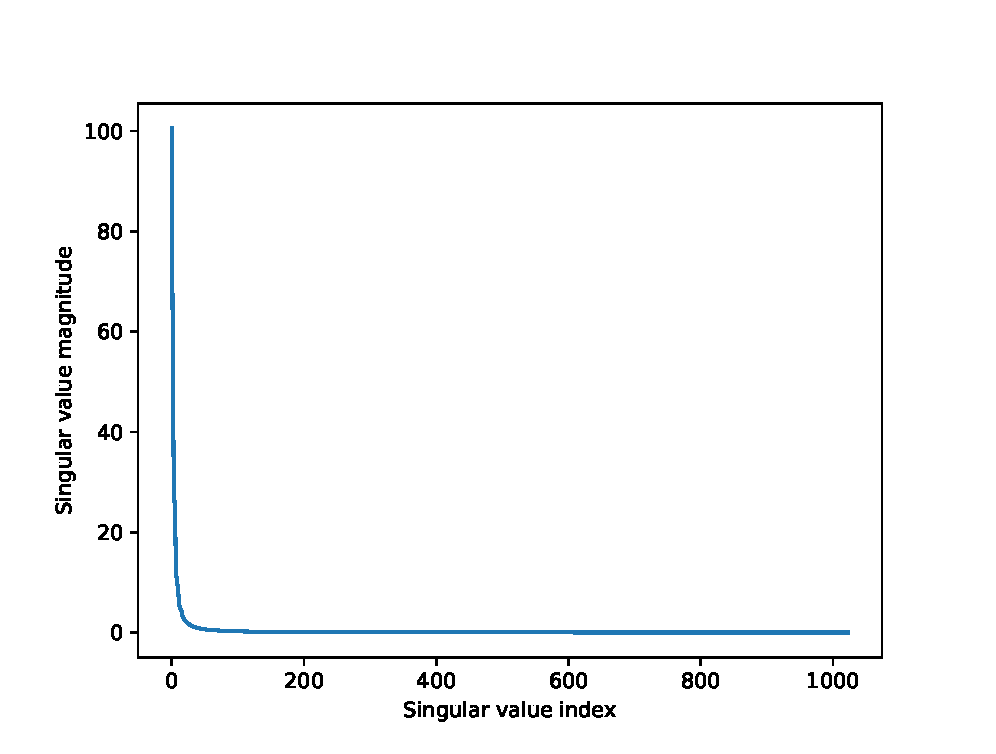
\includegraphics[width=0.6\linewidth, trim={0, 0.2cm, 0, 1.5cm}, clip]{singular_values.eps}
		\caption{Singular values of a 2D Gaussian random field}
		\label{fig:singular_values}
	\end{figure}
	
	We compute the best rank-20 approximation of this matrix using both truncated SVD and \maxvol{}-based pseudo-skeleton decomposition. The pseudo-skeleton had an error of about 2 times the SVD error in Frobenius norm, which is quite good, considering that the SVD approximation is the best possible. More importantly, the pseudo-skeleton decomposition was computed \textbf{thirty times faster} on average than the SVD, despite the fact that we used the highly optimized \texttt{np.linalg.svd} function to compute the SVD and used slow, high-level Python/\texttt{NumPy} code to compute the \maxvol{}-based pseudo-skeleton decomposition, suggesting that performance improvements of up to 100 times are likely possible.
	
	Pictured in Figure \ref{fig:reconstructions} are visualizations of the original Gaussian random field alongside the SVD and pseudo-skeleton approximations.
	\begin{figure}[h]
		\centering
		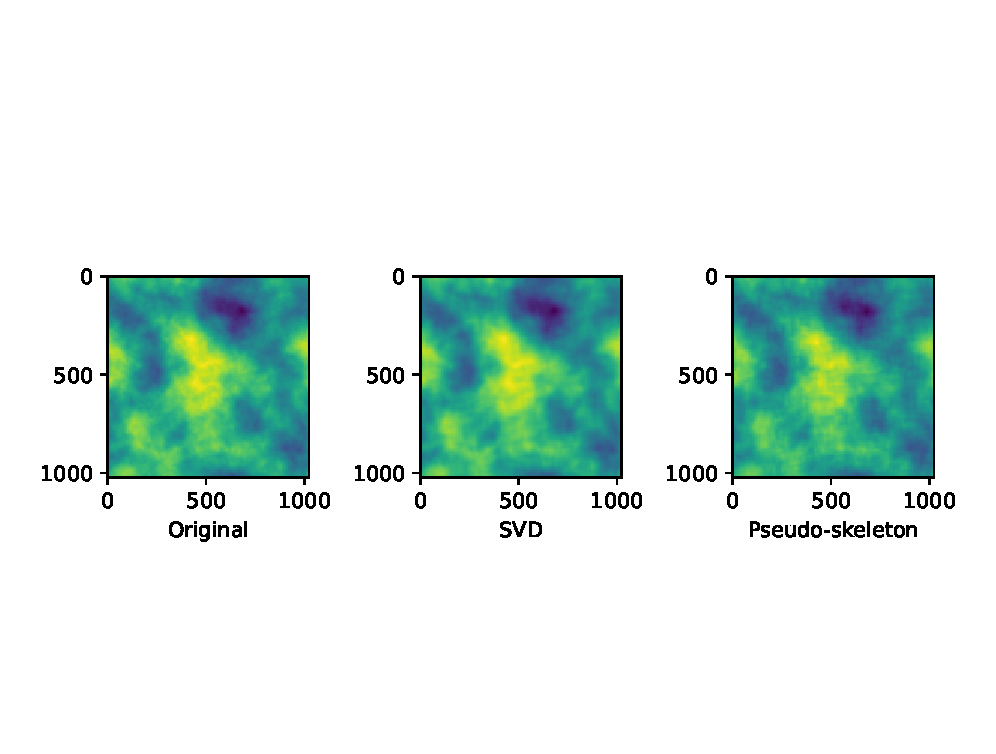
\includegraphics[width=\linewidth, trim={0, 3.25cm, 0, 4cm}, clip]{reconstructions.eps}
		\caption{Rank-20 approximations of a 2D Gaussian random field.}
		\label{fig:reconstructions}
	\end{figure}
	
	\minorheading{Fast optimization with \maxvol{}}
	
	The last experiment we did is taken from ``How to Find a Good Submatrix'' \cite{goreinov_2010}. In this experiment, we are given a large $m\times n$ matrix of (known) low rank $r$. We can use the alternating \maxvol{} method used to compute the pseudo-skeleton approximation to find a submatrix with high volume. Then, we find the largest element in absolute value of that submatrix. This element should approximate the largest element in absolute value of the given $m\times n$ matrix.
	
	To generate an $m \times n$ matrix of rank $r$, we choose the entries of matrices $U$ and $V$ of sizes $m\times r$ and $n\times r$ uniformly and random. Then, we take the QR decomposition of these matrices to obtain the Q factors $Q_U$ and $Q_V$ of full-rank. Lastly, we select the elements of a diagonal $r\times r$ matrix $D$ all positive and form the random $m\times n$ matrix $M = Q_UDQ_V^T$ of precisely rank $r$.
	
	Summarized in Table \ref{table:approximate_maxima} are the results of this experiment on several random $1000\times1000$ matrices. We see that the determined maxima are fairly close to the true maxima, in the sense that they are much better than guessing at random, as evidenced by the mean and standard deviation of the absolute value of elements of the generated matrices.
	\begin{table}
		\centering
		\begin{tabular}{@{}lllll@{}}
			\toprule
			Trial \# & True max & True mean & True std. & Approximate max\\
			\midrule
			1 & 0.003309 & 0.000451 & 0.000413 & 0.001745\\
			2 & 0.003262 & 0.000468 & 0.000360 & 0.002201\\
			3 & 0.003578 & 0.000514 & 0.000395 & 0.001665\\
			4 & 0.003420 & 0.000454 & 0.000350 & 0.002207\\
			5 & 0.003175 & 0.000480 & 0.000365 & 0.002400\\
			\bottomrule
		\end{tabular}
		\caption{Approximate maxima found using pseudo-skeleton decomposition}
		\label{table:approximate_maxima}
	\end{table}
	
	\section{Conclusion}
	
	Performing linear algebraic operations on matrices is a ubiquitous task, and, in many cases, the matrices involved are enormous. Reducing the size of a matrix by low-rank approximation is an effective way to make very slow or even infeasible computations much more accessible.
	
	Unfortunately, the theoretically optimal way to reduce the matrix size, truncated singular value decomposition (Theorem \ref{thm:svd}), may be as computationally expensive to perform as the task for which the matrix needs to be reduced in the first place. Therefore, it is desirable to have an algorithm that can find a reduced approximation of a matrix with complexity on the order of the size of the \textit{reduced} matrix, rather than the \textit{original} matrix. This essentially boils down to finding a good submatrix of the original matrix.
	
	We have shown that a good enough submatrix can yield an approximation that is nearly as good as truncated singular value decomposition. In the process of understanding this theory, we were led to the idea of maximum volume as the criterion for a good submatrix, and from there to the idea of the \maxvol{} algorithm. We showed that this algorithm is capable of finding a nearly maximal volume submatrix with a total number of computations on the order of the size of the submatrix, not the original matrix.
	
	Based on our experiments, we observed that \maxvol{} can provide a speedup of several orders of magnitude in the construction of low-rank approximations, and these approximations are of fairly high quality.
	
	As a final remark, we mention that the maximum volume idea can be extended readily to the more general area of \textbf{tensor decomposition}, which is the process of factorizing a tensor into the tensor product of other tensors. Much like how we used matrix decomposition to construct an efficient, low-rank representation of a matrix, tensor decomposition can be used to construct efficient, low-rank representations of tensors. Because the complexity of \maxvol{} depends primarily on the rank of the approximation, it can be used to overcome the curse of dimensionality by efficiently constructing low-rank approximations of high-dimensional tensors. The computational cost of operating on such an approximation scales linearly in the dimension (as opposed to the exponential scaling incurred by working on a dense, full-rank tensor).
	\bibliographystyle{plain}
	\bibliography{references.bib}
\end{document}